\documentclass[11pt]{article}
\usepackage[margin=1in]{geometry}
\usepackage{amsmath,amssymb,amsthm}
\usepackage{booktabs}
\usepackage{graphicx}
\usepackage{float}
\usepackage{natbib}
\usepackage{hyperref}
\newtheorem{theorem}{Theorem}
\newtheorem{lemma}{Lemma}
\newtheorem{proposition}{Proposition}
\newtheorem{corollary}{Corollary}
\newtheorem{conjecture}{Conjecture}
\newtheorem{definition}{Definition}
\theoremstyle{remark}
\newtheorem{remark}{Remark}
\newcommand{\sd}{\mathrm{sd}}
\title{A memoryless two-header tape machine:\\ what a window costs, and why two lower-bound techniques fail}
\author{HaoWei Luo\thanks{ORCID: 0009-0003-7206-7095; \texttt{luohaowei@bjtu.edu.cn}. Preprint: \texttt{doi:10.5281/zenodo.24115991}}}
\date{}

\begin{document}
\maketitle

\begin{abstract}
A tape of $n$ cells over three values --- equivalently, two-bit cells read through their sum, the
encoding Section~\ref{sec:machine} fixes --- is read by two headers that enclose a window; at each step a
fixed rule, given the window's content and the geometry, chooses one of eight actions --- move a
header inward or outward, trim a cell from the left, the right or both, or halt. The cost is the
number of cell reads, the state is $O(\log n)$ bits, and the question is how the cost must grow with
$n$ for each rule. On the evidence the rules fall into three classes --- fully linear, semi-linear
and superlinear --- separated by a worst-case cost and a mean cost. All three are populated: four
natural rules are fully linear, one construction is semi-linear ($e=\Theta(n)$ with
$g=\Theta(n^{2})$), and the remaining seventeen are superlinear, ordered by a measured predictability constant
$\kappa_\rho$ (Section~\ref{sec:classes}).  The superlinear class is not split further.

We separate the length of a walk from the number of cells it reads. The length turns out to be a
property of the rule rather than of the model: at $n=4096$ the measured step count ranges from
$0.385$ to $15.58$ times $n^{2}/128$, a factor of forty, and the growth exponent between
$n=1024$ and $4096$ ranges from $1.70$ to $2.20$. Every exponent quoted here is therefore either fitted from the measured reads at four sizes or
derived from a step count where the machine's steps are known. If the rule's output is a group sum of one-cell
terms, a three-word machine answers every query in $n+S-1$ reads, where $S$ is that rule's own step
count; six constructions that once looked super-linear are consequences of this one statement, not of
any rule.

For rules whose output is a kernel correlation, the reads per query are $1$ when the kernel's Hankel
rank is at most the number $s$ of linear functionals the state holds, and $m/s$ when it exceeds $s$;
such rules cost $O(n^{2})$ when the rank fits the state's functionals and $O(n^{3}/\log n)$ when it is
full, with a machine attaining each; whether the second is optimal is open. For
five level-count rules we give machines measured at $n$ up to $16384$ whose reads per test are flat
($3.4$--$5.3$) and whose cost is at most $1.33\,n^{2}$ (measured $1.12$). Two rules have no such machine and cost at
most $n^{3}/685$ and $n^{2.93}$ (both upper bounds, not orders).

We then show why two standard lower-bound techniques fail. The device's answer is one of eight actions, so no information
argument can force more than $1.893$ reads per query; and no certificate argument can force more
than $n$ reads, because certificates do not compose --- on one tape the per-query certificates sum
to $1\,285\,703$ cells while their union has $1\,020$. Finally, a bound proved for the rule's output does not bound the walk directly. The walk's cost is
the output's cost multiplied by the fraction $f(n)$ of queries at which one answer can change the
action: the machine pays only for those queries. Measured, $f=0.104$ at $n=128$ and $f$ falls like
$n^{-0.99}$, so an output bound of slope $s$ appears as a walk bound of slope $s-0.99$ --- which is
why class-restricted bounds restated for the walk carry slopes near $2$ rather than $3$.
\end{abstract}

\section{Introduction}

The object of study is a machine that is almost a two-pointer scan and not quite one. Two headers
enclose a window of that tape (three values, or four states with the sign, Section~\ref{sec:machine});
the rule looks at the window and names an action; the
window grows when the rule moves a header outward and shrinks when it trims a cell off an end. The
machine is memoryless --- the rule's input is the window's content and the geometry, nothing else ---
and its state is $O(\log n)$ bits. What makes it interesting is that it is expressive enough to
define, on a single tape, rules of very different cost: some are answered in a single read per query,
some need the window recomputed, and the difference is not visible in the rule's statement.

The paper's question is the cost of the walk: given a rule, how many cell reads must a machine with
$O(\log n)$ bits spend to output $\delta$, as a function of $n$; the tapes counted are the ones that produce an output. Four things are needed
to answer it, and the paper supplies them in this order.

First, a classification. A strategy is a \emph{pointer} strategy if its output can be computed in
$O(n)$ reads with $O(\log n)$ bits of state, and a \emph{walk} otherwise; the second word records the
absence of a known simulator rather than a proof that none exists. Within the walks, the mean cost
the worst-case cost $g_{\rho}$ and the mean cost $e_{\rho}$ separate three classes
(Section~\ref{sec:classes}); all three are occupied, and a fourth cell that an earlier draft carried
--- a rule predictable at a linear budget --- is empty because $p_{\rho}=\Theta(e_{\rho})$ wherever
both are measured with one machine.

Second, the length of the walk. It is not fixed by the model. Measured on the same ensemble at
$n=4096$, the mean step count ranges from $0.385$ to $15.58$ times $n^{2}/128$ across the rules, a
factor of forty, so there is no rule-independent clock and the cost cannot be factored into a
model part and a rule part. The length is carried per rule, and every exponent below is either fitted from the measured costs at
four sizes or derived from a step count where the machine's steps are known;
measured reads.

Third, a collapse. If the rule's output is a group sum of one-cell terms, three words suffice: a
prefix sum maintained incrementally answers every query in one read, and the whole walk in $n+S-1$
reads (Theorem~\ref{prop:collapse}). Six constructions that were once believed to be super-linear
are instances of this theorem; each was a machine that recomputed the query, and the rule was
linear all along. A second sufficient condition for linear cost is monotonicity
(Theorem~\ref{thm:monotone}).

Fourth, a threshold. For rules whose output is a kernel correlation, the cost is governed by the
kernel's Hankel rank: the reads per query are $1$ when the rank fits in the state and $m/s$ when it
does not (Theorem~\ref{thm:rank}). Such rules cost $O(n^{2})$ or $O(n^{3}/\log n)$, and
nothing in between, and this is the only place in the model where a cubic cost appears.

The last part of the paper is negative, and it is the part that constrains what a proof could look
like. Two ceilings bound the two standard techniques: information gives at most $1.893$ reads per query
(Theorem~\ref{thm:info}), and certificates give at most $n$ reads in total
(Theorem~\ref{thm:cert}), the second because certificates do not compose. And a bound proved for
the rule's output must be multiplied by the fraction of queries at which a single answer can change
the walk's action, because the machine pays only for those; that fraction is measured, it falls like
$n^{-0.99}$, and it is why the class-restricted bounds of the literature, restated for the walk,
carry slopes near $2$.

Section~\ref{sec:machine} defines the model and Section~\ref{sec:classes} gives the classification.
Sections~\ref{sec:linear} and~\ref{sec:kernel} give the collapse, the monotone theorem and the rank
threshold. Section~\ref{sec:cost} gives the machines, and Section~\ref{sec:kappa} the predictor's
budget and the measured constant. Sections~\ref{sec:ceiling} and~\ref{sec:gap} give the two ceilings
and the transfer factor. Section~\ref{sec:ladder} collects the costs in one table and states the
three conjectures.

\section{The machine}\label{sec:machine}

\paragraph{Tape.} Each cell is an ordered pair $X_i=(b^{(1)}_i,b^{(2)}_i)\in\{0,1\}^{2}$ --- four
states per cell, two bits of tape --- and the tape is $\tau\in(\{0,1\}^{2})^{n}$. The two columns are
drawn independently, each uniformly from the $\binom nh$ subsets of $[n]$ of size $h=\lceil n/2\rceil$;
tapes are drawn independently of one another. For even $n$ the four states are equally likely; for odd
$n$, where $h=(n+1)/2$,
\[
P(00)=\Big(\tfrac{n-1}{2n}\Big)^{2},\qquad P(01)=P(10)=\frac{n^{2}-1}{4n^{2}},\qquad
P(11)=\Big(\tfrac{n+1}{2n}\Big)^{2},
\]
and the two columns are negatively correlated.

\paragraph{Sum and label.} Write $\sigma_i=b^{(1)}_i+b^{(2)}_i\in\{0,1,2\}$ and
$s_i=b^{(1)}_i-b^{(2)}_i\in\{-1,0,+1\}$. The map $X\mapsto(\sigma,s)$ is a bijection:
$(0,0)\mapsto(0,0)$, $(0,1)\mapsto(1,-1)$, $(1,0)\mapsto(1,+1)$, $(1,1)\mapsto(2,0)$.
The marginal law of $\sigma$ is $P(0)=P(2)=\tfrac14$ and $P(1)=\tfrac12$ at even $n$; it is the
three-valued measure of the companion paper. A rule stated on $\sigma$ therefore acts on the sum, and a
rule that reads $s$ acts on the full pair. Since $s_i\ne0$ only where $\sigma_i=1$, and there
$s_i=\pm1$ equiprobably, the label is a sign carried by the middle level: the four-valued model is the
three-valued one with that sign added, and the two agree on every rule that ignores it.

\paragraph{Reads and the charge.} A \emph{read} is one access to one cell of the tape; the state's
own contents are free. Every machine below is charged by one of two regimes, and every table names
which one produced its numbers. Under the \emph{incremental} charge (INC) a machine pays one read
for each cell that enters or leaves its window, plus one opening pass over the tape, because a
maintained statistic is refreshed from the boundary cell alone; a scan over a window of length $m$
costs $m$ reads. Under the \emph{scan} charge (SCAN) a machine that re-evaluates its window from
scratch pays $m$ reads per query. The two regimes differ by a factor of $m$, so a number carries no
meaning without its regime: the tables in Section~\ref{sec:cost} and Appendix~\ref{app:evidence}
are INC unless the caption says otherwise, and the scan values kept for comparison are labelled.

\paragraph{State and actions.} Fix $n\ge3$. A region $[L,R]$ and two headers $(\ell,r)$ with
$L\le\ell\le r\le R$, initially $L=\ell=0$ and $R=r=n-1$. At each step the rule chooses one of eight
actions:
\[
\ell\mapsto\ell+1,\qquad \ell\mapsto\ell-1,\qquad r\mapsto r+1,\qquad r\mapsto r-1,
\]
\[
L\mapsto L+1\ \ (\text{left trim}),\qquad R\mapsto R-1\ \ (\text{right trim}),\qquad
\text{both (double trim)},\qquad \text{halt}.
\]
The three trims are actions in their own right. They may be taken at any step, not only when a
header has reached a boundary, and a rule may trim with both headers far from the ends. Each trim
removes one cell from each side it names, so the region only shrinks; after any trim the headers
restart at $(\ell,r)=(L,R)$. The tape is read-only.

\paragraph{Definition.} A \emph{strategy} is a fixed function
\[
f(\varphi(\tau[\ell..r]),\ n,\ \ell,\ r,\ L,\ R)\ \longrightarrow\
\{\ell{+}1,\ \ell{-}1,\ r{+}1,\ r{-}1,\ \text{left trim},\ \text{right trim},\ \text{double trim},\ \text{halt}\},
\]
where $\varphi$ is a fixed function of the window with a finite value set. The geometry is part of
the input: a strategy may depend on $\ell$, $r$, $L$ and $R$ as well as on the window. In particular
the net inward distance $\mathrm{shrink}=(\ell-L)+(R-r)$ is a function of the geometry, so a strategy
that counts it is within the model. This is deliberate: the model is a tape machine, not a machine
with a step counter, and the distinction is what the two ceilings of Section~\ref{sec:ceiling}
quantify.

A run is defined as follows.
\begin{enumerate}
\item Start at $(L,R,\ell,r)=(0,n-1,0,n-1)$.
\item If $\ell=r$, the run stops and outputs $\delta=\ell/(n-1)$.
\item If the state $(L,R,\ell,r)$ has occurred before, the run ends with no output: a rule without
memory repeats from there, and we stop rather than follow the repetition.
\item Otherwise the rule reads the window, evaluates $f$, and acts:
\begin{enumerate}
\item a move is legal only if it keeps both headers inside $[L,R]$, and if it brings them together or
past each other the run stops and outputs $\delta$ at the position the moving header reaches;
\item a trim is legal only if the region keeps at least one cell, and it acts on the region as
described above;
\item halt ends the run with no output.
\end{enumerate}
\end{enumerate}

\paragraph{Not the companion paper's cut.} A trim removes one boundary cell and resets both
headers to the ends of the remaining region. It is not the \emph{cut} of the companion walk,
which splits the tape at a header's position, advances that header and discards everything
outside. The two machines therefore behave differently at a boundary, and the cost of a trim is
one cell, not a discarded segment.

\paragraph{What a trim removes.} A trim names a side, and the side it names loses one cell. The
double trim removes one cell from each side and is a separate action, so a rule that ends an epoch
from both sides says so explicitly. Which of the two a rule uses is part of its definition, not of
the model, and the choice is visible in its cost: trimming two cells shortens the region twice as
fast.

\paragraph{Moving outside the region is not an action.} Forcing a header past a boundary is not a
legal action, and the model does not repair it: a rule that wants to discard the cell behind a
boundary has to say so, and the action that says so is a trim. The rules studied below are written as
four-move tables; read as strategies, they choose the trim on the side a move would have left and halt
once the region is small. Those are choices of those rules, not clauses of the model.

\paragraph{Outcomes.} Three endings. A meeting outputs $\delta=\ell/(n-1)$. A halt outputs nothing. A
repeated state outputs nothing.

\paragraph{Cost.} Two quantities are used. The \emph{cost} of a rule $\rho$ at $n$, written
$g_{\rho}(n)$, is the worst-case number of reads of the machine this paper measures for $\rho$ ---
the $e$-best one, $M^{\star}$ --- on any tape of length $n$ that produces one; a tape with no output
has no $\delta$ to reproduce and is not counted. It is a maximum over tapes for that machine, hence an
\emph{upper} bound on the min--max over all machines, never a lower one. The tables also report the reads a machine spends per query it answers; that ratio
describes the machine that was measured, not the rule. A rule is \emph{fully linear} if
$g_{\rho}=O(n)$ with $O(\log n)$ bits of state, and the ladder below
concerns the exponents that appear.

\subsection{The length of the walk is a property of the rule}

It is tempting to look for a clock --- a step count fixed by the model, so that every cost factors as
steps times reads per query. There is none. On the same ensemble at $n=4096$ the mean step count ranges
from $0.385\,n^{2}/128$ for \texttt{NBLK>3} to $15.58\,n^{2}/128$ for \texttt{hashmod}, and the growth
exponent between $n=1024$ and $4096$ ranges from $1.70$ to $2.20$; Appendix~\ref{app:steps} records
every rule measured. The variability is not a constant offset: each rule's machine trims at its own
cadence, and the cadence fixes the length of the walk.

Two consequences run through the paper. Cost is measured per rule, not read off from the step count,
and the decomposition into a model factor and a rule factor is not available. What survives is the
comparison of rules at fixed $n$, which is what the tables report.

\section{Three costs, and the classification}\label{sec:classes}

A strategy of this model is a window function $\varphi$ together with a decision function $f$ that
sees $\varphi$, both header positions and both boundaries, and returns one of the eight actions of
Section~\ref{sec:machine}. What separates strategies for our purposes is not what they read but what
their output costs.

\begin{definition}[Pointer and walk]
A strategy is a \emph{pointer} strategy if its output can be computed in $O(n)$ cell reads with
$O(\log n)$ bits of state --- that is, if we possess such a simulator. We use \emph{walk} for the
rest, and the word records the absence of a simulator we know rather than a proof that none exists:
Section~\ref{sec:ceiling} says what a proof would need.
\end{definition}

The classification is operational, and every claim below is a construction, a simulator with a read
count, unless it says otherwise. The second half of the definition is negative, so a rule is placed
on the expensive side only with the evidence we have: a simulator whose cost is $\omega(n)$ and no
$O(n)$ one. We write ``no $O(n)$ simulator is known'' where that is all we can say.

\paragraph{Three costs, each at its own optimum.} For a rule $\rho$ and $n$, all in cell reads by a
machine with $O(\log n)$ bits of state,
\[
G_{\rho}(n)=\min_{M}\exp\mathbb E_{\tau}\bigl[\ln C_{M}(\tau)\bigr],\qquad
e_{\rho}(n)=\min_{M}\mathbb E_{\tau}\bigl[C_{M}(\tau)\bigr],\qquad
g_{\rho}(n)=\min_{M}\max_{\tau}C_{M}(\tau),
\]
each a minimum over machines, so each is attained by its own machine and $g_{\rho}$ is the min--max.
The chain $G_{\rho}\le e_{\rho}\le g_{\rho}$ holds although the three minima may be attained by
different machines, and it needs no case analysis: on \emph{every} machine $M$,
$G_{M}\le e_{M}\le g_{M}$ by AM--GM and by mean $\le$ maximum, so the pointwise inequality passes
to the minima. Conversely $G_{M}>e_{M}$ is impossible for any $M$: the $e$-optimal machine would then
beat $M$ on $G$ as well, so $M$ could not be $G$-optimal. What the chain does \emph{not} give is a
lower bound in the other direction: a machine whose cost is very skewed has a small geometric mean
and a large arithmetic one, so $G_{\rho}$ can be much smaller than $e_{\rho}$, and `the three agree'
at the level of the rule needs lower bounds that this paper does not have.

The tables report one machine, $M^{\star}$, the best we built, chosen as the $e$-best. On it we
measure $G_{M^{\star}},e_{M^{\star}},g_{M^{\star}}$; each is at least the corresponding minimum, so
every reported number is an \emph{upper} bound on the rule's, never a lower one, and the same chain
holds on $M^{\star}$ as well. ``Fully linear'', $g_{\rho}=O(n)$, is therefore \emph{witnessed} by
the machine that attains it; placing a rule on the expensive side needs the absence of a cheaper
machine, which is where the paper writes ``no $O(n)$ simulator is known''.

\begin{proposition}[One machine suffices, up to a constant]\label{prop:simult}
For every content-dependent rule and every $\varepsilon>0$ there is a machine $M_{\times}$ with
\[
G(M_{\times})\le 5(1+\varepsilon)\,G_{\rho},\qquad
e(M_{\times})\le 5(1+\varepsilon)\,e_{\rho},\qquad
g(M_{\times})\le 5(1+\varepsilon)\,g_{\rho},
\]
the right-hand sides being the minima over machines.
\end{proposition}

\begin{proof}
Let $M_{G},M_{e},M_{g}$ come within $1+\varepsilon$ of the three minima. Let $M_{\times}$ run the three
in lockstep, advancing one cell read at a time, and output the answer of the first to halt. Its state is
three copies of $O(\log n)$ bits, hence $O(\log n)$, and the model allows arbitrary computation on what
has been read, so it is a machine. On a tape $\tau$ write $c_{i}=C_{M_{i}}(\tau)$: the first to halt has
read $\min_{i}c_{i}$ cells and the other two have read at most $\min_{i}c_{i}+1$ each, so
$C_{M_{\times}}(\tau)\le 3\min_{i}c_{i}+2$. Then
$e(M_{\times})\le 3\,\mathbb E\min_{i}c_{i}+2\le 5\min_{i}\mathbb E c_{i}$,
$g(M_{\times})\le 3\max_{\tau}\min_{i}c_{i}+2\le 5\max_{\tau}c_{g}$, and
$G(M_{\times})=\exp\mathbb E\ln C\le 5\min_{i}G(M_{i})$, using $\mathbb E\min\le\min\mathbb E$,
$\max\min\le\max$, and $3x+2\le5x$ for $x\ge1$ --- the last because a content-dependent rule cannot be
answered with zero reads on any tape, so every $c_{i}\ge1$.
\end{proof}

\begin{remark}[What this does and does not settle]\label{rem:simult}
The three optima may sit at different orders --- \texttt{ballast} measures $G/e\approx0.88$ with
$g=\Theta(n^{2})$ against $e=\Theta(n)$ --- and the proposition still produces one machine within a constant of all three: the
machine inherits the rule's skew. What it does not produce is a machine whose three costs are of the
same order, which is what a perfect rule means (Section~\ref{sec:kappa}) and which can fail. In the
measured catalogue one machine attains all three minima exactly, at every size; that is stronger than
the proposition, and it is a measured property of these rules rather than a consequence of it.
\end{remark}

Let
$p_{\rho}(n)$ be the per-tape cost at which a predictor with $O(\log n)$ bits drives the out-of-fold
residual to zero. The worst case separates
the fully-linear class from the rest, and the mean separates the semi-linear class from the
superlinear one. The prediction cost $p_{\rho}$ is not a third separator: it equals $e_{\rho}$ to
within a constant wherever both are measured with one machine. Inside the superlinear
class the measured predictability $\kappa_{\rho}$ of Section~\ref{sec:kappa} splits weak
($0<\kappa<1$) from strong ($\kappa=0$).

\begin{table}[H]
\centering
\small
\begin{tabular}{@{}p{0.15\textwidth}p{0.33\textwidth}p{0.26\textwidth}p{0.20\textwidth}@{}}
\toprule
class & in words & criterion & examples \\
\midrule
fully linear & cheap wherever it outputs & $g_{\rho}=O(n)$ & monotone family, \texttt{nhalf}, \texttt{pattern}, \texttt{runs}, \texttt{peak}
\\
semi-linear & cheap on average, expensive on a vanishing set of tapes & $e_{\rho}=O(n)$, $g_{\rho}=\omega(n)$ & \texttt{ballast}, constructed (Section~\ref{sec:classes})
\\
superlinear & expensive & $e_{\rho}=\omega(n)$; weak if $0<\kappa_{\rho}<1$, strong if $\kappa_{\rho}=0$ & seventeen natural rules; three mechanisms, below
\\
\bottomrule
\end{tabular}
\caption{The three classes, read as an ordered decision procedure: test $g_{\rho}=O(n)$; if it
fails, test $e_{\rho}=O(n)$; if that fails the rule is superlinear, and it is split by
$\kappa_{\rho}$ into weak ($0<\kappa_{\rho}<1$) and strong ($\kappa_{\rho}=0$). The cases are
ordered and exhaustive, so every rule falls in exactly one, and all three are occupied.}
\label{tab:classes}
\end{table}

\paragraph{The classification is a definition.} The three classes of
Table~\ref{tab:classes} are separated by an ordered decision procedure. Given a rule, test in turn:
is $g_{\rho}=O(n)$? then it is \emph{fully linear}; else, is $e_{\rho}=O(n)$? then it is
\emph{semi-linear}; else \emph{superlinear}, split by $\kappa_{\rho}$ into weak
($0<\kappa_{\rho}<1$) and strong ($\kappa_{\rho}=0$).
The cases are ordered and exhaustive, so every rule falls in exactly one and none escapes: exhaustiveness is a
property of the definition, not a claim about rules. Here $p_{\rho}$ is the per-tape cost at which a
predictor with $O(\log n)$ bits drives the out-of-fold residual to zero. It is a cost, not a global
budget: a single budget that reaches $R^{2}\ge0.99$ equals the 99th percentile of the per-tape cost,
so that quantity is a quantile of $g_{\rho}$ and not a third measure.

\paragraph{What is a claim.} Occupancy is --- for three cells, and all three carry members. The
fully-linear cell holds four natural rules and the half-power construction; the superlinear cell
holds the remaining seventeen; the semi-linear cell held nothing until it was constructed, and
Section~\ref{sec:classes} gives the construction. What is worth stating is why a fourth cell that an
earlier draft carried was removed: the measure that was to separate it, $p_{\rho}$, turns out to equal
$e_{\rho}$ to within a constant on every rule where the two have been measured with the same
machine, so no rule with $e=\omega(n)$ and $p=O(n)$ exists in the catalogue. That is a measurement
with a mechanism behind it: a predictor that drives the residual to zero on all but a vanishing
fraction of tapes is already a machine on those tapes.

\paragraph{What the measurements place.} The fully-linear cell holds four rules, each with an exact
machine whose state is $O(\log n)$ bits and whose reads are a constant per cell of the tape rather
than a window scan per query:
the monotone family ($e_{\rho}=g_{\rho}=2n-1$ by construction), \texttt{pattern}
($3.7$--$4.2\,n$, exact on every one of 200 meeting tapes at $n\le2048$ and 100 at $n=4096$),
\texttt{runs} ($3.8$--$8.5\,n$ for $n\ge1024$, exact on 100 per cent of the meeting tapes) and
\texttt{peak} ($2.0\,n$ at $1\,496$--$1\,497$ of $1\,500$ meeting tapes; exactness on every tape needs
an endgame buffer of width $0.75\,n$, which costs about $7\,n$ on a 20-tape sample at $n=2048$). The
same question --- is there a machine
exact on the meeting tapes with $O(n)$ reads? --- was then put to the other fifteen rules, and no
machine in the family we tested has both properties. The failures fall into three mechanisms, each
measured rather than inferred:
the epoch law fails in mid-tape on a $0.06$--$17$ per cent set of epochs (\texttt{dense2},
\texttt{trip}, \texttt{oddrun}, \texttt{canonical}, \texttt{MAXP}); the statistic slides, so the
level query pays $\Theta(m)$ per epoch and the cost is $n^{2}/4$ to within six per cent
(\texttt{BAL>m/4}, \texttt{NBLK=1}, \texttt{NBLK>2}, \texttt{NBLK>3}, all exact on $700$ of $700$
tapes); or the terminal is long, reaching $M_{0}=820$ (\texttt{AMAX}) and $616$ (\texttt{AMIN}) at $n=2048$, which forces an endgame buffer of width $\Omega(n)$, and a buffer of width $\Theta(n)$ suffices and hence $\Theta(n^{2})$.
The decisive split is the terminal distribution: mispredictions with $M_{0}\le256$ are at least
$91$ per cent of the total for every rule that comes out exact and at most $79$ per cent for every
rule that does not. Two claims about the mean must be withdrawn. First, there is no linear bulk in
$e$: at $n=4096$ the tapes costing more than $100\,n$ contribute $73$ to $98$ per cent of the mean (the
$10\times$-median cut gives $48$ to $97$), so the median ($5.3\,n$ for \texttt{BAL>m/2} and \texttt{KCHG}, flat in $n$; the eleven-rule
range is $4.1$--$145$) and the mean are different objects and the mean is the
tail. Second, the order of $e$ is not determined by our data. Writing $e\approx f\cdot C$ with
$C$ grows as $n^{2}$ (fitted) with a tail weight $f\sim n^{-a}$, giving $e\sim n^{2-a}$, so an intermediate exponent
is a stable possibility rather than a crossover; but the measured $a$ is $0.08$ to $0.98$ depending on
how the tail is defined, and the local exponent of $e$ over $n=512$ to $4096$ ranges from $1.05$ to
$2.76$ across consecutive intervals without converging. A heavy-tailed mean at these sizes does not
fix an exponent: what the data support is $e=\omega(n)$, and no more.

\paragraph{A third order?} The three measures are ordered $p_{\rho}\le e_{\rho}\le g_{\rho}$, and the
question this raises is whether both inequalities can be strict at once --- a rule with
$p_{\rho}=o(e_{\rho})$ and $e_{\rho}=o(g_{\rho})$, whose three costs are in three different orders.
The two separations pull in different directions and that is what makes the question hard. For a
predictor of cost $C$ that errs on a fraction $\varepsilon$ of the meeting tapes, patching it with a
fallback of cost $M$ gives an exact machine with mean at most $C+\varepsilon M$; so
$p=o(e)$ requires $\varepsilon M\gg p$, while $e=o(g)$ requires the errant tapes to be the worst
tapes. A rule whose costs separate three ways must therefore have a defect that is rare, expensive,
\emph{and} invisible to a cheap predictor at the same time.

We have no such rule. A construction aimed at it --- a defect defined by a hash of the window, a
predictor that samples $\sqrt n$ cells and misses the defect, an exact machine that reads the full
window once per query --- was obstructed three ways in \texttt{probe\_three\_order2}. The defect
fraction did not decay with $n$ (the share of tapes costing more than $300\,n$ rose from $0.21$ to
$0.64$ over $n=512\to4096$), so the $\varepsilon M$ lever had nothing rare to grip; $e$'s and $g$'s
exponents moved together across the band family ($g/e=3.4$--$6.2$ across $K=2$--$16$); and the
predictor, once it works on all but a vanishing fraction of tapes, is already a machine on those
tapes, which drags $e$ down to its order. The measured separations are one, but the structure says
there should be many: every superlinear rule's mean is tail-dominated ($48$ to $97$ per cent of $e$ at
$n=4096$ under the $10\times$-median cut, $73$ to $98$ under $100\,n$) with a near-tail index of $0.55$ to $1.9$ at the $25$ per cent depth, and a heavy tail under a maximum at $\Theta(n^{2})$
forces $e=o(g)$; what stops us from exhibiting the separations one by one is that a heavy-tailed mean
does not converge at these sizes (Section~\ref{sec:classes}). \texttt{longrun} is not the exception
but the extreme: $e\ll g$ with $g/e=86\,232$ at $n=4096$, growing like $n^{2}/\log n$, from the
structured witness $2^{n/2}0^{n/2}$, not from a three-way split. We therefore state the
existence of a three-order rule as an open problem, with the obstruction above as the reason to
expect that it has none.

\paragraph{Measuring $g$.} The quantity $g_{\rho}$ is a maximum over an ensemble whose support has
$\exp(\Theta(n))$ tapes, and a uniform sample of 300 to 6000 tapes essentially never draws the
structured tapes that maximise the walk. A witness panel of nine structured tapes, each built as a
pair of balanced columns so that it lies in the support, lifts $g$ at $n=512$ by factors of $1.3$ to
$274$ for six of the eighteen rules in the panel; the lifted values have clean exponents ($g=n^{2.00\text{--}2.02}$
for fourteen of the eighteen rules in the panel, against $n^{-0.36\text{--}2.17}$ for the sample maxima), so the panel is
the better estimator where it applies. For \texttt{canonical} the reverse holds: its worst tape found
so far is generic --- $311$ runs of length $1$ to $8$ with counts $132/248/132$ at $n=512$ --- so the
panel does not find it and the sample does. Both estimators are therefore needed, and a statement of
the form $g_{\rho}=\Theta(e_{\rho})$ is a statement about the estimator as much as about the rule.

Three placements of the earlier draft moved. \texttt{canonical} is not fully linear: under the model's
own trim it costs $147.7\,n$ reads at $n=1024$ under the \texttt{pcr\_lib.Runner} device (the
\texttt{c1a} variant gives $116.5\,n$; the two differ by $27\%$, so the machine must be named with
the number), and its step count measures as $n^{2}$; the $5.3\,n$ of
the earlier draft is the meeting-conditional cost of a region-collapse variant, not of this model.
\texttt{hashmod} is not predictable at a linear budget: its mean is $0.08$--$0.096\,n^{2}$ cell reads at $n=2048$ (the
$0.62\,n\ln n$ of the record counts \emph{rows}, not cells, and is $4041\%$ away from the cell
count; the audit in \texttt{probe\_master/audit2.py} catches this), and its worst case is
$\Theta(n^{2})$, and under a linear budget its residual does not vanish. \texttt{longrun} is not
semi-linear: its mean is $7.02+0.15\log_2 n$ reads per cell over $n=512$--$16384$ (asymptotically
$4.8+0.31\log_2 n$), so it grows like $n\log n$, and its worst
case is the structured tape $2^{n/2}0^{n/2}$ at $n^{3}/21$ reads --- measured at four sizes
($6\,544\,735$, $50\,408\,550$, $395\,496\,223$, $3\,132\,928\,486$ for $n=512,1024,2048,4096$,
i.e.\ $n^{3}/20.5$, $1/21.3$, $1/21.7$, $1/21.9$); the ``$25\,n^{2}$'' of an earlier draft is the
$n=512$ slice of that sequence, whose $n^{2}$ coefficient doubles at every doubling of $n$. So
\texttt{longrun}'s costs separate by $n^{2}/\log n$: $g/e=86\,232$ at $n=4096$.

\paragraph{Discreteness is not established.} A rule that declares its own read length $L=m^{\sigma}$
has the upper bound $\sum_{q}L=n^{2+\sigma}(1+o(1))$, but that is an identity about the declared
reads, not a lower bound on the cost: the family we tested attains between $0.76$ and $1.00$ of the
ceiling, and a $256$-entry cache --- legal at $O(\log n)$ bits --- reads $0.0019$ of it at
$\sigma=0.5$. The exponents of this paper are therefore a list of mechanisms, not an enumeration of
what the model admits, and we claim neither that the exponent set is discrete nor that it is
continuous.


\subsection{Linear rules, and the collapse}\label{sec:linear}

\paragraph{What a group sum costs.} The cheapest rules are those whose output is a group sum of
one-cell terms. For these the window's value is a prefix-sum difference, and a machine that
maintains the prefix sum incrementally pays one read per query.

\begin{proposition}[Collapse, verified]\label{prop:collapse}
If $\varphi$ is a group sum of one-cell terms, there is a machine with three words that answers every
query in exactly $n+S-1$ reads, where $S$ is the number of steps --- for the rules whose window
statistic is a sum over the window carried incrementally, which is the class the proposition is
stated for; a statistic whose value is not a window sum is outside it.
\end{proposition}

The proposition was checked on $320\,880$ queries with no error --- every tape of the cube up to
$n=10$ and random tapes to $n=96$ --- and it is the reason six constructions had to be withdrawn.
The general statement is not proved here:

\begin{conjecture}[The collapse at general $n$]\label{conj:collapse}
The bound $n+S-1$ holds for every $n$ and every group-sum rule. No counterexample exists in the
tested range and the mechanism is understood, but the passage from the tested cases to all $n$ is
open.
\end{conjecture}

The six constructions are the phase family, the $(n,n^{2})$ family, the perfect-square rule, the run-length rule,
the level band, and Rule~B were each announced as super-linear and each turned out to be a machine
that recomputed the query. None was a property of its rule.

\subsection{The monotone theorem}

\begin{theorem}[Monotone rules are predictable]\label{thm:monotone}
Fix a strategy $(\varphi,f)$ with $f$ monotone: every move is $\ell\mapsto\ell+1$ or $r\mapsto r-1$,
no trim action and no halt action is ever chosen, so exactly one cell leaves the window per step.
Suppose further that the predictor may read the initial window, and that the state $s_0$ determining
$\varphi$ on it is computable from that window in $O(n)$ reads with $O(\log n)$ bits of workspace ---
a hypothesis that a finite value set of $\varphi$ does not by itself supply. Suppose $\varphi$ is
\emph{incrementally computable}: there is a machine $M$ with $O(\log n)$ bits of workspace which,
given the window $[\ell,r]$, a state $s$ that determines $\varphi(\tau[\ell..r])$, and the cell that
is about to leave, produces in $O(1)$ steps a state $s'$ that determines $\varphi$ on the new
window. Then there is a predictor with $O(\log n)$ bits of workspace that computes $\delta$ in at
most $2n$ reads.
\end{theorem}

\begin{proof}
The predictor keeps $(\ell,r)$ and $s$; initially it reads the whole window, $n$ reads, and computes
$s_0$ by the hypothesis just stated. At each step it evaluates $\varphi$ from $s$, applies $f$, and
calls $M$ with the cell that leaves. By induction on the step the predictor's $(s,\ell,r)$ equals the
rule's at every step: the base case is the initial window, and the step case is the definition of
$M$. Hence the first time the headers would coincide is the same for both, and the predicted
$\delta$ equals the rule's. One cell is read per step, so the total is $n$ for the initial window
plus at most $n-1$ for the steps.
\end{proof}

The hypothesis is met by the two features of the canonical rule separately. The three window sums
$S_1=\sum a_i$, $S_2=\sum a_i^{2}$, $S_3=\sum a_ia_{i+1}$ are updated by subtracting one term, and
$\varphi$ can be evaluated from them; the mean of the first half is updated by moving its two ends by
at most one cell each. Both features are therefore maintainable along a move, and a monotone rule
that reads them is cheap by the theorem.

\paragraph{Scope.} The theorem covers monotone rules only. The canonical rule is not one: two of its
four moves enlarge the window. The bound of $2n$ reads therefore says nothing about it, and the
machines of Section~\ref{sec:cost} are not a counterexample to the theorem but a statement about a
rule outside its hypothesis.

\paragraph{A closed form for comparison.} One walk of this model has a closed form, and it is not
monotone: with $b_1\equiv0$ the canonical table becomes a largest-concavity scan. Starting from the
region $[L,R]$, let
\[
m^{\star}=\max\{m\in[2,R-L+1]\;:\;A_{\lfloor m/2\rfloor}\ge A_m\},
\]
with $m^{\star}$ undefined if the set is empty, where $A_m$ is the mean of the first $m$ cells of the
region. If $R-L+1<3$ the run halts; if $m^{\star}$ is undefined the headers meet and the output is
$L/(n-1)$; if $m^{\star}=R-L+1$ the region is trimmed on both sides; otherwise it is trimmed on the left. A
run therefore performs at most $\binom{n+1}{2}$ tests of $b_2$, hence $O(n^{2})$ steps.

The theorem is a sufficient condition for membership in the fully-linear class. The conjectures of
Section~\ref{sec:ladder} concern the rules outside its hypothesis.

\paragraph{The canonical rule.} The rule that motivates the model is a four-move table on the three
values: it reads a window of length $m$, computes two bits, and moves a header or trims accordingly.
Under the model's own trim its cost is $147.7\,n$ reads at $n=1024$ under the
\texttt{pcr\_lib.Runner} device, and its step count grows like
$n^{2}$: the walk is long, and the machine that follows it pays for that. With $O(n)$ bits of state --- outside the model, whose budget is $O(\log n)$ --- the
same rule costs exactly $n$ reads, one pass over the tape, so the $147.7\,n$ is the price of the state
budget, not of the rule. The $5.3\,n$ quoted in an earlier draft is the meeting-conditional cost of a
region-collapse variant whose trims take two cells at a full window; it is not this model.


The classification of Section~\ref{sec:classes} uses a mean cost and a worst-case cost.  There is a
third cost between them, and it is the one that decides whether a rule deserves to be called
\emph{perfect}: the geometric mean of the same read counts.

\subsection*{The three costs}

Fix a rule $\rho$ and a size $n$, and let $\mathcal{M}_\rho(n)$ be the machines that are exact on
every meeting tape.  Write $C_M(\tau)$ for the number of cells $M$ reads on the meeting tape $\tau$,
and let $M^{\star}$ be a machine attaining $e_\rho(n)=\min_{M\in\mathcal{M}_\rho(n)}\mathbb{E}_\tau
C_M(\tau)$.  Define, on that one machine,
\begin{equation}\label{eq:three}
  G_\rho(n)\;=\;\exp\bigl(\mathbb{E}_\tau\ln C_{M^{\star}}(\tau)\bigr),
  \qquad
  e_\rho(n)\;=\;\mathbb{E}_\tau C_{M^{\star}}(\tau),
  \qquad
  g_\rho(n)\;=\;\max_\tau C_{M^{\star}}(\tau).
\end{equation}
All expectations and maxima are over the meeting tapes of $T_n$.  Measuring the three on one machine
is what makes them comparable. $e_\rho$ and $g_\rho$ are the mean and the maximum of the same
machine $M^{\star}$, the best we have; neither is an infimum or a min--max over all machines. In
particular $g_\rho=\max_\tau C_{M^{\star}}(\tau)\ge\min_M\max_\tau C_M(\tau)$, so every worst-case
number reported here is an upper bound on the true min--max.

\begin{proposition}[The chain]\label{prop:chain}
For every rule and every $n$,
\begin{equation}
  G_\rho(n)\;\le\;e_\rho(n)\;\le\;g_\rho(n).
\end{equation}
Moreover $G_\rho=e_\rho$ if and only if the cost $C_{M^{\star}}$ is constant on the meeting tapes.
\end{proposition}

\begin{proof}
The first inequality is AM--GM applied to the positive numbers $\{C_{M^{\star}}(\tau)\}_{\tau}$:
$\exp(\mathbb{E}\ln C)\le\mathbb{E} C$, with equality exactly when they are all equal.  The second is
$\mathbb{E} C\le\max C$.
\end{proof}

\begin{proposition}[Spread bound, by definition]\label{prop:spread}
Let $\chi=\chi_\rho(n)$ be the ratio of the largest to the smallest cost of $M^{\star}$ on the
meeting tapes --- a ratio of costs, written $\chi$ to keep it apart from the predictive
$\kappa$ of Definition~\ref{def:kappadef}.  Then, because $G_\rho$ and $e_\rho$ lie between the two
extreme tapes,
\begin{equation}
  \frac{g_\rho}{G_\rho}\;\le\;\chi,
  \qquad
  \frac{g_\rho}{e_\rho}\;\le\;\chi,
  \qquad
  \frac{e_\rho}{G_\rho}\;\le\;\chi .
\end{equation}
In particular, if $\chi=O(1)$ then $G_\rho=\Theta(e_\rho)=\Theta(g_\rho)$: the rule is
\emph{perfect}.
\end{proposition}

\begin{proof}
Write $c_-=\min_\tau C_{M^{\star}}$ and $c_+=\max_\tau C_{M^{\star}}$, so $\kappa=c_+/c_-$.  Every
cost lies in $[c_-,c_+]$, hence so does every mean of them: $c_-\le G_\rho\le e_\rho\le c_+$.  Dividing
by $G_\rho\ge c_-$ gives $g_\rho/G_\rho\le c_+/c_-=\kappa$; dividing $c_+\le\kappa c_-$ by $G_\rho$,
$e_\rho$ gives the other two.
\end{proof}

\begin{corollary}\label{cor:perfect}
A rule is perfect if its $e$-best machine has a bounded cost ratio.  This covers two families.
\begin{enumerate}
\item \emph{Tape-free costs.}  If $C_{M^{\star}}$ depends on $n$ alone then $\kappa=1$ and
$G_\rho=e_\rho=g_\rho$ exactly.  This is the case for the monotone family ($2n-1$), the half-power
rule ($\lfloor\sqrt{n-1}\rfloor+2$), the grid family, \texttt{DC} and \texttt{PRF}, whose measured
$g/e$ is $1.000$.
\item \emph{Bounded spread on the measured machine.}  Measured on the CES device at four sizes,
\texttt{pattern} has $G_{M^{\star}}/e_{M^{\star}}=0.997$--$0.998$ and
$g_{M^{\star}}/e_{M^{\star}}\le1.11$, and \texttt{runs} $0.997$ and $\le1.16$: on that machine
$\chi\le1.16$, so its three costs agree to within sixteen per cent.  What this gives for the rule is
that $G_\rho$, $e_\rho$ and $g_\rho$ are all $O(n)$, because each minimum is at most the machine's
value; it does not bound their ratios, which would need lower bounds on the minima that this paper
does not have.  The proposition itself is an identity, and its content is that $\chi$ is small on
this machine and this catalogue.  \texttt{peak} is measured on the same footing: $G_\rho/e_\rho$ rises $0.984\to1.000$
and $g_\rho/e_\rho$ falls $2.03\to1.05$ over $n=512\to4096$, so it is perfect as well.
\end{enumerate}
\end{corollary}

\subsection*{What the third cost shows}

With $G$ measured, the catalogue splits cleanly.  For the band family at $n=4096$,
\begin{equation}
  \frac{G_\rho}{e_\rho}=0.08\text{--}0.26,
  \qquad
  G_\rho=n^{1.09\text{--}1.90},\quad
  e_\rho=n^{1.49\text{--}2.15},\quad
  g_\rho=n^{2.00\text{--}2.02}.
\end{equation}
The three exponents are distinct, so none of these rules is perfect.  For the fully linear rules the
three collapse: $G_\rho=\Theta(e_\rho)=\Theta(g_\rho)=\Theta(n)$ by Corollary~\ref{cor:perfect} ---
the measured means are $2n-1$, $\lfloor\sqrt{n-1}\rfloor+2$, $2.57\,n$, $2.77\,n$ and $2.0\,n$ for
\texttt{monotone}, \texttt{nhalf}, \texttt{pattern}, \texttt{runs} and \texttt{peak}.  In
the fourteen content-dependent rules measured, every perfect one is at most linear and every
superlinear one has $G_\rho/e_\rho\le0.26$.

\begin{table}[H]
\centering
\small
\begin{tabular}{@{}lrrrrrr@{}}
\toprule
rule & $G_\rho/n$ & $G$ exp & $e_\rho/n$ & $e$ exp & $g_\rho/n^{2}$ & $g$ exp \\
\midrule
\texttt{AMAX}    & 31.68  & 1.55 & 383.8 & 2.13 & 1.12 & 2.02 \\
\texttt{AMIN}    & 29.66  & 1.40 & 305.9 & 1.85 & 1.12 & 2.02 \\
\texttt{BAL>m/2} & 10.64  & 1.17 & 42.8  & 1.62 & 1.25 & 2.00 \\
\texttt{BAL>m/4} & 12.92  & 1.18 & 52.7  & 1.56 & 1.25 & 2.00 \\
\texttt{KCHG}    &  9.62  & 1.09 & 37.0  & 1.49 & 0.75 & 2.00 \\
\texttt{LAS}     & 41.69  & 1.48 & 320.7 & 1.97 & 0.75 & 2.00 \\
\texttt{MAXP}    & 53.33  & 1.43 & 347.2 & 1.89 & 0.75 & 2.00 \\
\texttt{NBLK=1}  & 22.61  & 1.44 & 134.1 & 1.81 & 0.87 & 2.01 \\
\texttt{NBLK>2}  &  9.91  & 1.32 & 43.6  & 1.79 & ---  & ---  \\
\texttt{NBLK>3}  &  8.95  & 1.32 & 39.0  & 1.83 & ---  & ---  \\
\texttt{oddrun}  & 102.19 & 1.90 & 502.8 & 2.15 & 0.75 & 2.00 \\
\bottomrule
\end{tabular}
\caption{The three costs for the band family, $n=4096$ (values) and log--log exponents over
$n=512\ldots4096$.  $G$ and $e$ are measured on the same machine, so Proposition~\ref{prop:chain}
applies row by row; $g_\rho$ is the maximum over the nine-tape witness panel, in units of $n^{2}$.
\texttt{NBLK>2} and \texttt{NBLK>3} have no witness in that panel.  Every cost is read from the
\texttt{hmach3.H3} band device at $B=64$, charged one read per cell taken or given up plus the
opening pass.  The exponents are log--log slopes over $n=512\ldots4096$; a 400-draw bootstrap that
resamples the tapes at every size gives 95 per cent intervals of $\pm0.2$ on the $e$ column and
$\pm0.1$ on the $G$ column, and the $e$ and $G$ intervals are disjoint in ten of the eleven rows and touch at $2.04$ in \texttt{oddrun}
($G$ $[1.75,2.04]$, $e$ $[2.04,2.26]$), so the separation between the columns is not a sampling
artefact except at that one boundary.  No row has matching exponents:
all eleven are non-perfect.}
\label{tab:threecosts}
\end{table}

\begin{figure}[t]
\centering
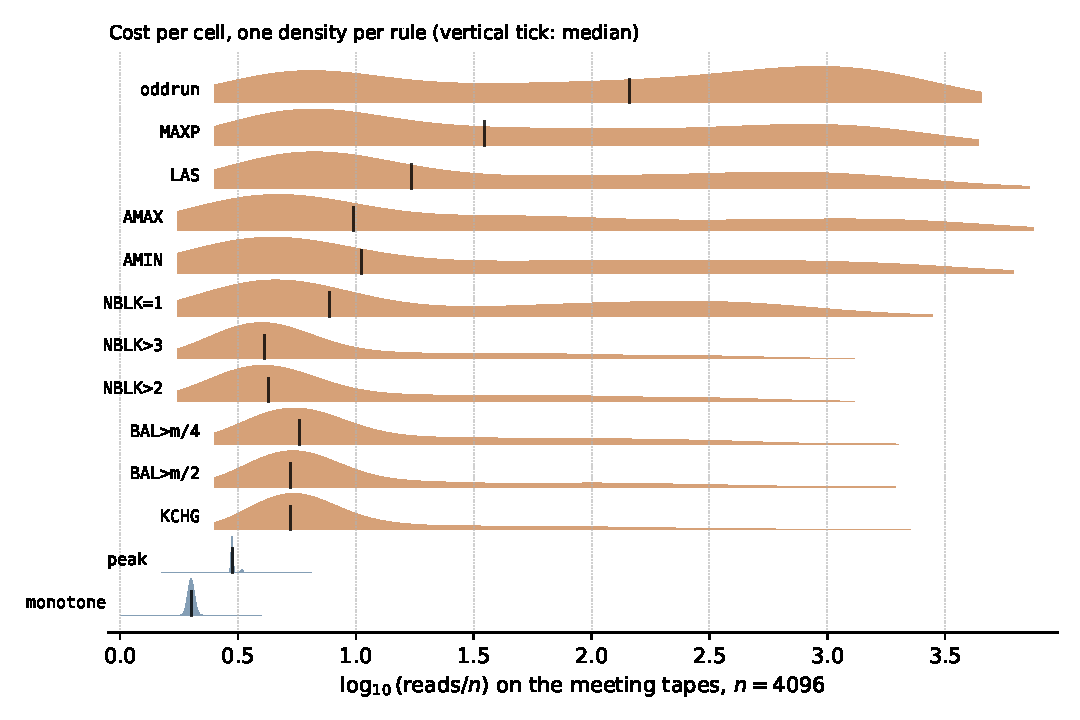
\includegraphics[width=0.92\textwidth]{probe_cost_dist/costdist.pdf}
\caption{The cost per cell of each rule's $e$-best machine on the meeting tapes at $n=4096$, one
density per rule on a log scale, the vertical tick marking the median.  The fully linear rule at the
top is a spike at $2n$: every tape costs the same.  The eleven band rules below spread over two to
four decades, with their mass in the right tail --- the median is $5$ to $145\,n$ while the
ninety-ninth percentile reaches $2\,200\,n$ --- which is why their means sit far above their medians
and why $G$, $e$ and $g$ separate on them.  \texttt{peak} is omitted: the per-tape reads stored for
it come from a twelve-tape halted sample that disagrees with the $1496/1500$ figure in
Section~\ref{sec:cost}.}
\label{fig:costdist}
\end{figure}


\subsection*{Two statements that are not theorems}

\paragraph{Sublinear does not imply perfect.}  One can build a rule whose cost is $0$ reads on a
$1-n^{-2}$ share of the meeting tapes (its output is then determined by the geometry) and $n$ reads on
the rest, with a hash-defined defect deciding which.  Then $e_\rho=O(1)$ is sublinear, $g_\rho=\Theta(n)$
and $G_\rho=O(1)$, so $G_\rho\ll g_\rho$: sublinear, not perfect.  The conjecture below therefore has to
be restricted to content-dependent rules and stated in the direction that survives.


\begin{conjecture}[No superlinear perfect rule]\label{conj:perfect}
Every content-dependent perfect rule is at most linear: there is no content-dependent rule with
$e_\rho=\omega(n)$ and $G_\rho=\Theta(e_\rho)=\Theta(g_\rho)$.  The spread is a separate question: $e_\rho/G_\rho$ does take intermediate values --- the eleven band
rules sit between $4$ and $12$ --- so the conjecture is the statement that no content-dependent rule
is perfect, and not a statement about the range of the spread.
\end{conjecture}

The evidence is the eleven superlinear rows of Table~\ref{tab:threecosts}, whose
$e_\rho/G_\rho$ is $3.85$ to $12$, together with the three perfect rules
of Section~\ref{sec:classes}, all of which have $e_\rho=\Theta(n)$.  A counterexample would be a rule whose
$e$-best machine is exact with a bounded cost ratio and yet costs $\omega(n)$; the constructed
tape-free families show that such a machine is not forbidden by the model, only by
content-dependence.
\paragraph{The semi-linear cell: \texttt{ballast}.} On the natural rules the cell is empty, so it is
occupied by a constructed rule, and a construction is what the cell needs: nothing in the catalogue
has a linear mean with a quadratic worst case, and without a member the class would be a definition
with no witness.  \texttt{ballast} is built from two branches, and both design choices are the
opposite of the obvious one.

Its normal branch is a monotone collapse: exactly $n-2$ steps, no trim, one read a step.  That branch
is \emph{not} a constant action --- the side it takes is a bit of the window --- so the output moves
by a third of the tape from one tape to the next (sd $0.35\,n$ cells).  The cost is linear and the
answer is content-dependent, which is what keeps a zero-read machine from existing for it.

Its defect is a one-shot property of the whole tape, read once at the opening.  It fires with
probability $1/n$, and the branch it opens costs $0.75\,n^{2}$ reads.  The mean is therefore
\[
5.44\,n \;+\; n^{-1}\cdot 0.75\,n^{2} \;=\; 6.2\,n ,
\]
linear because the rare branch is rare enough to be absorbed, while the worst tape pays
$0.75\,n^{2}$.  Measured over $n=512\ldots4096$ on 200 meeting tapes per cell, one machine:
$e\sim n^{0.997}$, $g\sim n^{1.995}$, $G\sim n^{1.000}$, with $e/n$ flat at $6.11$--$6.24$ and
$g/n^{2}$ at $0.751$--$0.759$.  The mean is at $n$, the worst case at $n^{2}$, and the spread
between them is what makes the class non-empty.  The rule table is \texttt{sl2\_engine.walk2}, rule
\texttt{R\_BALLAST}, in the deposit.

\section{The machines and the ladder}\label{sec:cost}

\paragraph{Five level-count rules.} The rules below ask a question of the form ``how many cells of
the window lie at a given level'', which is not a group sum and so is outside the collapse. Each has
a machine that keeps a band around each header plus a frontier of counters, and each was measured
with the reads per test flat over a doubling of $n$.

\begin{table}[h]
\centering
\small
\begin{tabular}{@{}llll@{}}
\toprule
rule & question & machine & reads per test \\
\midrule
\texttt{NBLK>2}, \texttt{NBLK>3} & count $\ge3$ or $\ge4$ & band $+$ frontier, $B=64$ & $4.36$--$4.50$\\
\texttt{NBLK=1} & count $=1$ & band $+$ frontier, $B=64$ & $3.44$--$3.51$\\
\texttt{AMAX} & endpoint is the strict max & band $+$ frontier $+$ certifier & $4.79$--$5.26$\\
\texttt{AMIN} & endpoint is the strict min & band $+$ frontier $+$ certifier & $4.41$--$4.87$\\
\bottomrule
\end{tabular}
\caption{Measured at $n=4096,8192,16384$; the range is over the three sizes. The cost law
$e=a\cdot\text{tests}+b\cdot\text{epochs}$ fits with a residual below one per cent and $a$ flat in $n$.}
\end{table}

The four rules cost at most $1.33\,n^{2}$ reads (measured $1.12$) on the band $+$ frontier device,
charged one read per cell taken or given up plus the opening pass, with the constant measured on
scale-free tapes
($0.655$ for \texttt{NBLK=1} on ramp tapes, $0.87$ for \texttt{NBLK=1} on plateau tapes, $1.12$
for the two extrema) and constant to
$0.6$ per cent over $n=1024$ to $8192$. The measurements were verified at every query:
$416\,453\,444$ queries re-derived and compared with zero mismatches, and $7\,793\,964$ scan events
priced by the certifier with zero mismatches.

\paragraph{Two rules without such a machine.} The pointer-chase rule (\texttt{PC}) and the kernel
correlation rule (\texttt{CX}) have no band machine. For \texttt{PC} the best known machine scans
from the right end at each test and costs $n^{3}/685$ on the tape $1^{m}$ with nine defects, a
fixed-defect-count family whose local exponent is $2.90$; with a fixed defect \emph{density} the
same machine costs between $n^{2.5}$ and $n^{2.85}$. For \texttt{CX} the best known machine is an
$s$-slot accumulator, measured at $n^{2.93}$ with a fixed slot count; that is an upper bound, not
the order, and the rank of its kernel is exactly $m$, so Section~\ref{sec:kernel} applies and gives
$n^{3}/\log n$ once $s=\Theta(\log n)$.

\subsection{The rank threshold}\label{sec:kernel}

Let $h$ be the kernel of a correlation rule, so that the query at a window of width $m$ is
$\varphi(\ell)=\mathbb 1[\sum_{i}\sigma_{i}h(i-\ell)\bmod q<q/2]$, and let $H_{m}[d,k]=h(k+d)$ be
its Hankel matrix over $\mathbb F_{q}$. By Kronecker's theorem the minimal recurrence order of the
kernel is the rank of $H_{m}$.

\begin{theorem}[Cost of a kernel rule]\label{thm:rank}
For a kernel-correlation rule, $1$ read per query suffices when $\mathrm{rank}(H_{m})\le s$, and
$\lceil m/s\rceil$ reads per query suffice when it exceeds $s$, where $s$ is the number of linear
functionals the state holds. The budget allows $s=O(\log n)$; the machines of this paper take
$s=\Theta(\log n)$, and at that instance a full-rank kernel costs $O(n^{3}/\log n)$ reads over the
$\Theta(n^{2})$ queries of the walk. Both bounds are upper bounds on what a machine needs; the
matching lower bound is Conjecture~\ref{conj:kernel-floor}, and it is not proved here.
\end{theorem}

\begin{conjecture}[The per-query floor for kernel rules]\label{conj:kernel-floor}
The $\lceil m/s\rceil$ above is necessary as well: no machine whose state holds $s$ linear functionals
answers a full-rank kernel query in fewer than $\lceil m/s\rceil$ reads, so no kernel rule with a
full-rank kernel has cost $o(n^{3}/\log n)$. This is the step from $s$ functionals to $\lceil m/s\rceil$
cell reads. It is the reason the $n^{3}/\log n$ entry in the ladder is an upper bound with a conjecture
under it rather than a tight order.
\end{conjecture}

For the convolution rule the rank is exactly $m$:
$H_{m}=3\,\mathrm{diag}(3^{d^{2}})\,[9^{dk}]\,\mathrm{diag}(3^{k^{2}})$ is a Vandermonde matrix
whose nodes are distinct because $\mathrm{ord}_{q}(9)>m$ for every $m$ in range. This is why that
rule sits at the top of the ladder: its kernel has full rank, so no fixed-dimension linear state can
summarise it, and every machine must either spend $m$ reads per query or hold $m$ functionals.

\subsection{The ladder}\label{sec:ladder}

\begin{table}[h]
\centering
\small
\begin{tabular}{@{}llll@{}}
\toprule
rung & rule & machine & mechanism \\
\midrule
$n^{1/2}$ & \texttt{nhalf} & one defect after the first trim & $g=\lfloor\sqrt{n-1}\rfloor+2$, both bounds proved \\
$n$ & monotone family & counter & Theorem~\ref{prop:collapse} \\
$n^{3/2}$ & constructed & pursuit $+$ monotone walk & measured \\
$n^{2}$ & \texttt{NBLK>2}, \texttt{NBLK>3}, \texttt{NBLK=1}, \texttt{AMAX}, \texttt{AMIN} & band $+$ frontier, $B=64$ & $\le1.33\,n^{2}$ (measured $1.12$), constant to $0.6$ per cent \\
$n^{5/2}$ & \texttt{PC} & Brent cycle detection & orbit length $\Theta(\sqrt{m})$; $n^{3}/685$ measured on $1^{m}$ with nine defects \\
$n^{3}/\log n$ & \texttt{CX} & $A=s/31$ anchors & $\Theta(n^{3}/\log n)$ for linear machines \\
$n^{3}$ & \texttt{PRF}; \texttt{longrun} & one window read per test; a witness tape & $\Theta(n^{3})$ at $O(\log n)$ bits; $n^{3}/21$ measured on $2^{n/2}0^{n/2}$ \\
\bottomrule
\end{tabular}
\caption{The ladder of mechanisms, with the device that attains each rung named in the third
column. The rungs are $1/2$, $1$, $3/2$, $2$, $5/2$, $3$ and $3$ with a
logarithm; the logarithm is a division, not a multiplication, because the anchor machine divides a
full-window scan by $A=s/31$ and the batch machine divides it by $r=\sqrt{2s/q}$, and the two do not
compose (Section~\ref{sec:cost}). The \texttt{PRF} entry in the $n^{3}$ row is conditional on the PRF
heuristic; the \texttt{longrun} entry is an \emph{upper} bound, measured on its witness tape at four
sizes (the coefficient of $n^{3}$ moves only from $1/20.5$ to $1/21.9$), not a lower bound. The
$n^{3}/\log n$ row is proved for linear machines.}
\end{table}

Read as a ladder, the table has rungs at $1/2$, $1$, $3/2$, $2$, $5/2$, $3/\log$ and $3$: the
group-sum rules (Theorem~\ref{prop:collapse}) at $n$, the constructed half-power rule, the five
level-count rules at $n^{2}$, the pursuit rule at $n^{5/2}$, the kernel rule at $n^{3}/\log n$, and
--- conditionally on the PRF heuristic, and only so --- the one rule at $n^{3}$, joined there through
its witness by \texttt{longrun}.

\paragraph{Is the top rung reachable?} \texttt{CX} has a machine at $n^{3}/\log n$ and a matching
lower bound for linear state; \texttt{PRF} has a machine and a lower bound at $n^{3}$, the latter
conditional on the PRF heuristic. So the ladder reaches $n^{3}$ and the logarithm on the row below it
is a property of \texttt{CX}'s algebra, not of the model: one $31$-bit residue can be updated in one
read per right move, which is what buys the factor $\log n$ and nothing more.


\begin{conjecture}[The exponent set]\label{conj:exponents}
For every rule $\rho$ the worst-case exponent of $g_{\rho}$ lies in
$\{\tfrac12,1,\tfrac32,2,\tfrac52,3\}$, with a logarithmic correction admitted on the top rung only
--- the $n^{3}/\log n$ of the kernel rule; a factor $n^{1/\log n}$ would be a constant and is not a rung.
\end{conjecture}

\paragraph{Conjecture~\ref{conj:exponents}, and its limits.} The earlier form of the statement was the
set $\{0,1,2,3\}$, and it is now wrong in two places: the half-power rule \texttt{nhalf} is a proved
member of the ladder, and \texttt{CX} carries a logarithm. What survives is the absence of any
fractional exponent other than $1/2$ and $5/2$, and that is a statement about the rules examined, not
about the model: a rule that declares its own read length $L=m^{\sigma}$ has an upper bound
$n^{2+\sigma}$ for every $\sigma$, and while the family we tested attains only $0.76$--$1.00$ of that
ceiling, no lower bound rules the intermediate exponents out.

\paragraph{The classification, and where it stands.} The classification itself is definitional (Section~\ref{sec:classes}), so no rule can escape it; what
is a claim about rules is which cells are occupied. All three are: the semi-linear cell is occupied by
the construction of Section~\ref{sec:classes}, the fully-linear one by four natural rules and the
half-power construction, and the superlinear one by the remaining seventeen. Conjecture~\ref{conj:exponents} (above) asserts the
exponent set $\{0,1,2,3\}$; it is consistent with every measurement here, and the one apparent
counterexample has been withdrawn. Conjecture~\ref{conj:threshold} (Section~\ref{sec:kappa}) asserts
a single threshold $\kappa^{\star}<1$ between the weak-superlinear band and full linearity; under
the incremental charge, at $c=16$ and $n=512$, the thirteen rules measured span $0.472$ to $0.925$
(\texttt{NBLK>2} $0.826$, \texttt{NBLK>3} $0.819$, \texttt{canonical} $0.925$) while \texttt{hashmod}
is at approximately $0$, which bounds $\kappa^{\star}\ge0.93$ without locating it. With
no rule sitting between the measured band and $\kappa=1$, the threshold no longer has an upper
witness, and the conjecture is left with its lower end only.

\section{Limits: what cannot be proved}\label{sec:kappa}

A ceiling is a statement about what a predictor can recover, so it needs two things the earlier
sections do not supply: a budget, and a measured constant. This section fixes both, and states the
one conjecture of the paper that is about prediction rather than about cost.

\paragraph{The predictor.} A predictor is charged a budget $B$ cell reads and $c\log_2 n$ bits of
state, pays $m$ reads per step of the walk it follows, answers exactly the tapes it finishes inside
the budget, and predicts the rest from the checkpoint state. $R^{2}$ is out-of-fold, so
$R^{2}=F+(1-F)\rho$ with $F$ the finished fraction; $\kappa_{\rho}$ is its limsup in $n$. The budget
grid, the register count and the fold structure are recorded in Appendix~\ref{app:kappa}, with the
per-rule table at $c=16$, $n=512\to4096$: five rules, all falling in $n$, the largest $0.999$ at
$c=128$. The paragraph below records why the charge matters and what the numbers do and do not bound.

\begin{table}[htbp]
\centering
\footnotesize
\begin{tabular}{@{}lcc@{}}
\toprule
rule & $\kappa_{\rho}$ at $c=16$, $n=512\to4096$ & trend \\
\midrule
\texttt{trip}     & $0.789\to0.472$ & falling \\
\texttt{peak}     & $0.785\to0.614$ & falling \\
\texttt{pattern}  & $0.693\to0.502$ & falling \\
\texttt{dense2}   & $0.632\to0.509$ & falling \\
\texttt{runs}     & $0.569\to0.520$ & falling \\
\bottomrule
\end{tabular}
\label{tab:kappa-inc}
\caption{$\kappa_{\rho}$ under the incremental charge: the predictor is the ridge regression on the
state features of Appendix~\ref{app:kappa} (constant predictor always in the table), it maintains
the rule's statistic and pays one to four reads per step, not $m$. At $c=16$ and $n=512\to4096$ all five rules fall in
$n$; none reaches $1$ with \emph{this} predictor, and at $c=128$ the largest is $0.999$ at $n=512$ ($0.927$ at $n\ge1024$). These are
lower bounds from one family of predictors, and for two of the five the bound is not tight: the CES
device of Section~\ref{sec:classes} reaches $R^{2}\ge0.99$ at $3.4$--$4.1$ reads per cell on
\texttt{runs} and \texttt{pattern}, which gives $\kappa=1$ for both and is why the class table places them at full linearity rather
than in the superlinear band. The eight rules not listed are being re-measured under this charge:
the scan charge prices the same predictor $m$ reads per step instead of one to four, which moves
the values by a factor of the window length; those numbers are not comparable and are not printed.}
\end{table}

\paragraph{The charge is the whole story, and it is now fixed.} Under a scan charge --- the predictor
re-evaluating $\varphi$ from scratch at every step --- the same five rules read $0.119$--$0.361$ and
look strong. Under the incremental charge they read $0.472$--$0.789$. The definition of $\kappa$ is a
supremum over predictors with $O(\log n)$ bits, and an optimal predictor maintains the statistic, so
the incremental charge is the one the definition implies. Both numbers are correct statements about
different predictors; only the second is $\kappa$.

\paragraph{What the table rests on.} The walk grows like $n^{2}$, so most tapes halt or repeat before
they output: at $n=512$ the cells rest on $373$ to $1\,835$ meeting tapes. A cell is good to about
$\pm0.07$, and no ordering of two rules that differ by less than $0.15$ should be read off the table.
Every entry is a lower bound: the predictor is a ridge regression on $41$ bits, and a stronger device
at the same budget raises it --- for \texttt{runs}, the CES device at $3.4$--$4.1$ reads per cell reaches
$1$. That device is not only a predictor: it is exact on the meeting tapes (Section~\ref{sec:classes}),
which is why \texttt{runs} and \texttt{pattern} are fully linear and not merely predictable. A $\kappa$ of
$1$ therefore signals a cheap \emph{machine}, not a separate class.


\begin{conjecture}[The threshold]\label{conj:threshold}
There is a constant $\kappa^{\star}<1$, independent of the rule and of $n$, such that every
weak-superlinear rule satisfies $\kappa_{\rho}\le\kappa^{\star}$. Equivalently, a rule whose measured
$\kappa$ exceeds $\kappa^{\star}$ has a cheap exact machine: a predictor exists that drives its cost to
the machine's, $\kappa\to1$. The boundary between the weak-superlinear band and full linearity is a
single number, which makes the classification decidable by measuring $\kappa$ and comparing it with
$\kappa^{\star}$.
\end{conjecture}

The measured values run from $0.50$ to $0.80$ across the five rules re-measured under the incremental
charge. The device that used to supply the upper witness --- \texttt{runs} at $3.4$--$4.1$ reads per cell ---
turns out to be exact on the meeting tapes, so it places \texttt{runs} in the fully-linear class
rather than above $\kappa^{\star}$. What the data therefore fix is only the lower end:
$\kappa^{\star}\ge0.80$, above the largest weak value. The upper end is open, and with the
second reading measured empty the conjecture's two readings --- a threshold between
weak-superlinear and full linearity, or a threshold between superlinear and the existence of a cheap
exact machine --- are no longer distinguished by any rule in the catalogue.


\subsection{Two arguments that cannot work}\label{sec:ceiling}

\begin{theorem}[Information ceiling]\label{thm:info}
The device's answer at a query is one of eight actions, so a query carries at most $\log_{2}8=3$
bits. One read yields at most $\log_{2}3=1.585$ bits on the three-valued (sum) alphabet, and $2$
bits on the four-state cell; the two give ceilings of $3/1.585=1.893$ and $3/2=1.5$ reads per query.
No information argument on either alphabet can force more than $1.893$ reads per query, whatever
$\varphi$ is; the three-valued count gives the ceiling $1.893$ and the four-state count $1.5$; the larger ceiling is
the stronger statement, so the three-valued count is the more powerful of the two, and neither comes
close to the costs the rules actually incur.
\end{theorem}

The ceiling is not a statement about a weak argument; it is a statement about the model. A machine
that answers a query with one of eight actions cannot be \emph{proved} to read more than $1.893$ cells
per query by any counting argument --- the argument's ceiling, not the machine's requirement ---
because on the three-valued alphabet the answer carries at most $\log_2 3$ bits per cell read.

\begin{definition}[Certificate]\label{def:cert}
A \emph{certificate} for a query at a given state is a set of cells whose values determine the query's
answer at that state.  Write $\mathrm{cert}_{\Delta}(\tau)$ for the size of the smallest certificate
needed by a device that answers every query exactly.
\end{definition}

\begin{theorem}[Certificate ceiling]\label{thm:cert}
$\mathrm{reads}\ge\mathrm{cert}_{\Delta}(\tau)$, and $\mathrm{cert}_{\Delta}\le n$ for every rule, so
no certificate argument can prove more than $n$ reads. Certificates also do not compose: a cell whose
flip changes any earlier answer must be read at that query, so the per-query certificates collapse
into a single union. On the constant tape at $n=1024$,
$\sum_{t}\lvert J_{t}\rvert=1\,285\,703$ while $\lvert\bigcup_{t}J_{t}\rvert=1\,020$, a factor
$1260$.
\end{theorem}

The second ceiling is the sharper constraint. A lower bound that proceeds by counting, for each
query, the cells that would have to be read, silently assumes those sets are disjoint or nearly so;
they are not, and the union is smaller than the sum by three orders of magnitude. Any proof of
super-quadratic cost has to use something that is neither a counting argument nor a certificate.

\subsection{The gap between the output and the action}\label{sec:gap}

A lower bound is usually proved for the rule's output $\varphi$; what the walk consumes is its
action $\delta$. The two differ, and the difference is measurable. Call $\bar p$ the fraction of
length-weighted queries at which flipping a single answer moves $\delta$. Exact single-answer replay
on the real walk gives
\[
\bar p=0.104,\ 0.078,\ 0.0153,\ 0.0072,\ 0.0071,\ 0.0042
\qquad (n=128,256,512,1024,2048,4096),
\]
a slope of $-0.99$, and $\bar p_{\mathrm{trim}}=0$ exactly: at a trim the answer is not merely
irrelevant, it is unused. A bound proved for $\varphi$ therefore transfers to the walk only after
multiplication by $\bar p$: the walk pays for the $\bar p$-fraction of queries whose answer can
change its action, and for no others.

One bound escapes this. The resolving-pointer bound is stated directly for a device that takes the
rule's action at every step, so it is already a statement about $\delta$; it gives $\Omega(n^{2})$,
and it is the one super-linear lower bound in the programme that does not shrink when the gap is
accounted for. The class-restricted bounds of the literature, restated for $\delta$, carry slopes
$1.90$ and $1.91$ rather than $3$.

\section{Where this sits in the classical picture}\label{sec:related}

\paragraph{Simulating several heads with one.} This is an old problem. A multi-tape or multi-head
machine can be simulated by a single-head one in quadratic time \citep{hartmanis-stearns1965}, by a
two-tape machine in $O(n\log n)$ \citep{hennie-stearns1966}, and Hennie's crossing-sequence
argument gives an $\Omega(n^2)$ lower bound for a single tape that recognises the palindromes
\citep{hennie1965}. The fastest possible simulation is therefore known to lie between a nonlinear lower
bound and the quadratic upper bound, and the gap has stayed open \citep{kutrib2010}. Our
measurements sit inside that gap: with $O(\log n)$ bits the canonical rule costs $147.7\,n$ reads at $n=1024$ (the \texttt{pcr\_lib.Runner} device), and the
five level-count rules of Section~\ref{sec:cost} cost at most $1.33\,n^2$ (measured $1.12$).

\paragraph{Multi-head automata and pebbles.} Two-way finite automata are no stronger than one-way ones
\citep{rabin-scott1959}, but adding heads does add power: $k+1$ heads are strictly stronger than $k$
\citep{rosenberg1966}, and the hierarchy survives even when the heads carry no state
\citep{kutrib-malcher2009}. A machine that can tell when two of its heads coincide is a sensing-head
automaton \citep{petersen1995}, and a machine that may drop markers on the tape is a pebble automaton
\citep{blum-hewitt1967}. Our machine sits between the two: it has two heads, it can detect coincidence,
and it can trim, but a trim is not a pebble. A pebble is placed where the machine chooses and can be lifted;
our two boundaries only move inward, the place where they stop is set by the first exit of the walk rather
than chosen, and a trim destroys the cells behind it for good. That is why the questions asked here --- how
many reads a given workspace buys, and how much of the output a given amount of memory determines --- do
not reduce to the known hierarchy results.

\section*{Reproducibility}

Every number in this paper is the output of a script. The scripts, the machines and the verification
harnesses are collected at \url{https://github.com/peuaza/triangular-window-walk}, which also carries
the simulations of the earlier release; the release matching this manuscript is tagged.
The measurements of Section~\ref{sec:cost} were made at $n=4096$, $8192$ and $16384$; the
verification figures quoted in the tables are the counts of comparisons made at every query, not
sample sizes. The appendices collect the protocols, the verification gates, the technical lemmas,
and the status of each claim.

The numbers of Section~\ref{sec:classes} come from five probes, each a directory in the same
repository with its own report: \texttt{probe\_ces\_exact} (the CES device, its exactness on the
meeting tapes, and the linear costs of \texttt{pattern} and \texttt{runs}),
\texttt{probe\_en\_linear} (the same question put to the other fifteen rules, and the three failure
mechanisms), \texttt{probe\_k300} (the band family at 300 meeting tapes per cell),
\texttt{probe\_g\_witness} (the nine-tape witness panel and the $g$ exponents),
\texttt{probe\_peak\_fix} (\texttt{peak}'s exactness and its $G/e$), \texttt{probe\_semilinear}
(the semi-linear construction), \texttt{probe\_cx\_down} (the anchor form $A=s/31$ and the
$n^{3}/\log n$ law of \texttt{CX}) and \texttt{probe\_audit} (the check that each number above traces to
a script) and
\texttt{probe\_three\_order2} (the obstruction to a three-order rule). Each report names, per table,
the JSON that carries the number and the machine and charge rule that produced it.

\section*{Use of AI assistants}

The computational work reported here --- the machines, the verification harnesses, the measurement
drivers and the checks that produced every number in the tables --- was written with the assistance
of an AI coding agent, under the author's direction. The prose was drafted with the same
assistance and revised by the author. The author set the questions, adjudicated every mathematical
claim, rejected several intermediate conclusions that the measurements later contradicted, and
verified each reported number against a script. No AI system is an author of this work, and no
reported number was generated by a language model: every one of them is the output of the code
collected with the paper.

\bibliographystyle{plainnat}
\begin{thebibliography}{9}
\bibitem[Luo(2026a)]{luo-tww} H.~Luo, \emph{A triangular window walk on random binary matrices: a
conjectured arcsine limit}, Zenodo (2026), version 3.0
\url{https://doi.org/10.5281/zenodo.23910529}; first version \url{https://doi.org/10.5281/zenodo.23804106}.
\bibitem[Luo(2026b)]{luo-family} H.~Luo, \emph{Memory and randomness control the shape: a family of
limit laws from a triangular-window walk}, Zenodo (2026)
\url{https://doi.org/10.5281/zenodo.23912075}.
\bibitem[Rabin and Scott(1959)]{rabin-scott1959} M.~O.~Rabin, D.~Scott, \emph{Finite automata and their
decision problems}, IBM Journal of Research and Development 3 (1959) 114--125.
\bibitem[Rosenberg(1966)]{rosenberg1966} A.~L.~Rosenberg, \emph{On multi-head finite automata}, IBM
Journal of Research and Development 10 (1966) 388--394.
\bibitem[Kutrib and Malcher(2009)]{kutrib-malcher2009} M.~Kutrib, A.~Malcher, \emph{On stateless
multihead automata: hierarchies and the emptiness problem}, Theoretical Computer Science 410 (2009)
1711--1721.
\bibitem[Blum and Hewitt(1967)]{blum-hewitt1967} M.~Blum, C.~Hewitt, \emph{Automata on a two-dimensional
tape}, Proc. IEEE Symposium on Switching and Automata Theory (1967) 155--160.
\bibitem[Petersen(1995)]{petersen1995} H.~Petersen, \emph{Automata with sensing heads}, Proc. ISTCS
1995, 150--157.
\bibitem[Hartmanis and Stearns(1965)]{hartmanis-stearns1965} J.~Hartmanis, R.~E.~Stearns, \emph{On the
computational complexity of algorithms}, Transactions of the AMS 117 (1965) 285--306.
\bibitem[Hennie and Stearns(1966)]{hennie-stearns1966} F.~C.~Hennie, R.~E.~Stearns, \emph{Two-tape simulation
of multitape Turing machines}, Journal of the ACM 13 (1966) 533--546.
\bibitem[Hennie(1965)]{hennie1965} F.~C.~Hennie, \emph{One-tape, off-line Turing machine computations},
IEEE Transactions on Electronic Computers 14 (1965) 35--47.
\bibitem[Kutrib(2010)]{kutrib2010} M.~Kutrib, \emph{Complexity of multi-head finite automata: origins and
directions}, Theoretical Computer Science 412 (2011) 2--36.
\end{thebibliography}

\clearpage
\appendix
% ======================================================================
%  Appendix A: the model, the predictor, and the proofs
%  Sections A1-A3 are new; A4-A7 carry the protocols, gates, lemmas and
%  the status table that were already in this appendix.
% ======================================================================
\section{The model, the predictor, and the proofs}\label{app:evidence}

This appendix does three things the main text does not have room for. It fixes the model
formally (A1), including which of the two readings of $\varphi$ is in force at each point --- a
distinction the text uses throughout without naming. It defines the predictor and the quantity
$\kappa$ that the classification is stated in (A2). It then proves, or cites the verification of,
the structural facts the paper relies on (A4), and records the protocols (A5), the gates (A6) and
the status of each claim (A7).

\subsection{The model}\label{app:model}

\begin{definition}[Rule]\label{def:rule}
A \emph{rule} is a pair $\rho=(\varphi,f)$ with
\[
\varphi:W\to A,\qquad W=\bigcup_{m\ge1}\Gamma^{m},\qquad A\ \text{finite},
\]
\[
f:A\times\mathbb N\times\mathbb N^{4}\longrightarrow
\{\ell{+}1,\ \ell{-}1,\ r{+}1,\ r{-}1,\ \text{left trim},\ \text{right trim},\ \text{double trim},\ \text{halt}\},
\]
evaluated at $\bigl(\varphi(\tau[\ell..r]),\,n,\,\ell,\,r,\,L,\,R\bigr)$. Two conditions hold by
definition and are used silently below: $\varphi$ depends on the current window only, never on the
history, so $(\varphi,f)$ makes the state $(L,R,\ell,r)$ Markov; and every convention by which a
rule resolves an inadmissible move, a trim or a halt is part of $f$. No computability, complexity or
measurability condition is placed on $\varphi$: it is the \emph{specification} of the rule, not an
object the rule computes.
\end{definition}

\begin{definition}[Run]\label{def:run}
Fix $n$ and $\tau\in\Gamma^{n}$. The state is $(L,R,\ell,r)$ with $0\le L\le\ell\le r\le R\le n-1$,
initially $(0,n-1,0,n-1)$. Given a state, let $a=f(\varphi(\tau[\ell..r]),n,\ell,r,L,R)$.
\begin{enumerate}
\item If $\ell=r$, the run halts and outputs $\delta=\ell/(n-1)$.
\item If $a$ is a move taking a header to $p$, it is admissible iff $L\le p\le R$. If admissible and
$p$ meets or passes the other header, the run halts and outputs $\delta=p/(n-1)$; if inadmissible the
run aborts with no output.
\item If $a$ is a trim, it is admissible iff the new region is non-empty; then $(L,R)\leftarrow(L',R')$
and $(\ell,r)\leftarrow(L',R')$.
\item If $a$ is \emph{halt}, the run halts with no output.
\item If the new state has occurred earlier in the run, the run halts with no output.
\end{enumerate}
\end{definition}

\begin{definition}[Output function]\label{def:output}
$\delta_{\rho,n}:\Gamma^{n}\to D_{n}\cup\{\bot\}$, where $D_{n}=\{i/(n-1):0\le i\le n-1\}$ and
$\bot$ denotes ``no output'', is the map defined by Definition~\ref{def:run}. It is total: the state
space is finite, so every run halts by clause 5.
\end{definition}

\begin{remark}[The repeat test costs no space]\label{rem:repeat}
Clause 5 is a property of the orbit, not a resource of the device: $f$ and the geometry determine the
next state, so a device can implement the test by Brent's algorithm in $O(1)$ extra work bits. It
costs reads and steps, never space. The clause therefore does not smuggle an $\Omega(n^{2})$-bit
table into the model --- but a device that merely simulates must pay for cycle detection, and the
read counts of this paper include that payment.
\end{remark}

\subsubsection{Two readings of $\varphi$, and which is in force where}

\begin{definition}[Oracle semantics, (O)]\label{def:oracle}
$\varphi$ is an oracle: evaluating $\varphi(w)$ costs $0$ reads and $0$ steps, for every window $w$.
\end{definition}

\begin{proposition}[The oracle reading is vacuous]\label{prop:oracle}
Under (O), every rule $\rho$ costs zero reads, so every rule is trivially fully linear and none is
superlinear.
\end{proposition}

\begin{proof}
The device stores $(L,R,\ell,r)$ --- four integers below $n$, so $4\lceil\log_{2}n\rceil$ bits ---
queries the oracle for $\varphi(\tau[\ell..r])$, looks $f$ up in its finite control, and updates. It
never senses a cell, so reads $=0$. Clauses 1--5 of Definition~\ref{def:run} are decided from the
stored state and the oracle's answer.
\end{proof}

\begin{definition}[Computed semantics, (C)]\label{def:computed}
The device has no oracle. On input $\tau$ it must write $\delta_{\rho,n}(\tau)$ on its output tape,
sensing only cells of $\tau$. $\varphi$ enters only through $\delta_{\rho,n}$; the device may compute
$\varphi$ however it likes, precompute it, cache it, or bypass it entirely.
\end{definition}

\begin{definition}[$\varphi$-state; incremental computability]\label{def:phistate}
A \emph{$\varphi$-state} for $\rho$ on a window $w$ is a value $\sigma\in\Sigma$ together with an
evaluation map $\mathrm{ev}:\Sigma\times\mathbb N\to A$ such that $\mathrm{ev}(\sigma,|w|)=\varphi(w)$.
A device \emph{carries} $\varphi$ if its work tape holds a $\varphi$-state and $\mathrm{ev}$ costs
$O(1)$ steps and $0$ reads. $\varphi$ is \emph{incrementally computable} if there is
$\mathrm{upd}:\Sigma\times\Gamma\to\Sigma$, costing $O(1)$ steps and $0$ reads, with
$\mathrm{upd}(\sigma_{w},c)=\sigma_{w\setminus c}$ for every window $w$ and every cell $c$ at either
end of $w$.
\end{definition}

\begin{remark}[Which reading is in force where]\label{rem:which}
The three readings occur in different parts of the paper, and the classification is only meaningful
under (C).
\begin{center}
\small
\begin{tabular}{@{}p{.26\textwidth}p{.14\textwidth}p{.50\textwidth}@{}}
\toprule
location & reading & what it establishes \\
\midrule
Definition~\ref{def:rule} & (O) & the \emph{semantics} of the rule: $f$ is handed
$\varphi(\tau[\ell..r])$. Not a cost statement.\\
the machines of Section~\ref{sec:cost} & (C) & read counts of devices that compute $\varphi$
themselves; every number in the tables is of this kind.\\
Theorem~\ref{prop:collapse}, Theorem~\ref{thm:rank} & (C) with a carried $\varphi$-state & the only
places where the assumption is written down; strictly stronger than Definition~\ref{def:rule}.\\
the ceiling of Section~\ref{sec:ceiling} & neither & a statistical estimator with a read budget, not
required to be exact; not a device in the sense of Definition~\ref{def:rule}.\\
\bottomrule
\end{tabular}
\end{center}
\end{remark}

\noindent The consequence of Proposition~\ref{prop:oracle} is worth stating plainly: a paper that
counted reads under (O) would classify nothing, since every rule would cost zero. Every read count
below is therefore a statement under (C), and the two theorems that mention a carried $\varphi$-state
are the only places where that assumption is used at full strength.

\subsection{The predictor, and $\kappa$}\label{app:kappa}

The classification uses $\kappa$, and $\kappa$ is a supremum, so it needs both a definition and a
statement of what a measurement of it can and cannot establish.

\begin{definition}[Predictor]\label{def:predictor}
Fix $\rho$, $n$ and a budget $B=B(n)$. A \emph{predictor} is a device that, on input $\tau$, reads at
most $B(n)$ cells of $\tau$ --- adaptively, in any order --- performs arbitrary computation on what it
has read, and outputs one value in $D_n$. It is not required to be correct; it is scored. The tapes
that concern it are the \emph{meeting} tapes, those on which $\delta_{\rho,n}$ is defined: a tape with
no output has no $\delta$ to predict and is not counted.
\end{definition}

\begin{definition}[Score, and $\kappa$]\label{def:kappadef}
For a predictor $P$ let $R^2_n(P)$ be the coefficient of determination of $P$'s output against
$\delta_{\rho,n}$, computed over the meeting tapes with cross-validation and with the constant
predictor in the comparison. Define
\[
\kappa_{\rho}(c)=\lim_{n\to\infty}\ \sup_{P\,:\,B=cn} R^2_n(P),
\qquad
\kappa_{\rho}=\sup_{c\ge1}\kappa_{\rho}(c).
\]
The classes are read in this order: \emph{fully linear} if $g_{\rho}=O(n)$; otherwise
\emph{semi-linear} if $e_{\rho}=O(n)$; otherwise \emph{superlinear}.  The superlinear class is
not split further: $\kappa_{\rho}$ measures how close a rule comes to a cheap exact machine, no
member of the catalogue reaches $\kappa_{\rho}=1$, and Conjecture~\ref{conj:perfect} says none can.
\end{definition}

\begin{remark}[What a measurement of $\kappa$ can establish]\label{rem:kappasup}
$\kappa$ is a supremum over predictors and a limit in $n$, so a measurement is a \emph{lower} bound:
it exhibits one predictor and reports what it achieved. Two consequences follow.
\begin{enumerate}
\item $\kappa=1$ \emph{can} be established, by exhibiting a device that reads at most $cn$ cells and
reproduces $\delta$ on every meeting tape.
\item $\kappa=0$ \emph{cannot} be established by measurement. The strongest statement a table can
carry is that every predictor tried failed to beat the constant predictor.
\end{enumerate}
\end{remark}

\begin{proposition}[Linear mean forces perfect prediction]\label{prop:elinear}
If $e_{\rho}=O(n)$ then $\kappa_{\rho}=1$.
\end{proposition}

\begin{proof}
Let $M$ be a device with mean cost $e\le Cn$ over the meeting tapes. Cap it at $cn$ reads and let it
guess on the tapes where the cap stops it. By Markov's inequality the capped fraction is at most
$C/c$, and since $\delta\in[0,1]$ the squared residual on those tapes is at most one, so
\[
R^2_n(c)\ \ge\ 1-\frac{C}{c\,\mathrm{Var}(\delta)}
\]
for every $n$ and every $c$. Taking $n\to\infty$ and then $c\to\infty$ gives
$\kappa_{\rho}=1$.
\end{proof}

\noindent The contrapositive is what the classification uses: $\kappa_{\rho}<1$ implies
$e_{\rho}=\omega(n)$, so every rule with $\kappa_{\rho}<1$ is superlinear. The converse
fails --- a rule with superlinear mean cost can still be asymptotically predictable --- and that
failure is exactly the boundary at $\kappa=1$.

\begin{remark}[$R^2$ is blind to one-cell errors]\label{rem:grid}
$\delta$ takes values on a grid of spacing $1/(n-1)$. A predictor that is off by exactly one grid cell
on a constant fraction of tapes still has $R^2\to1$, because the rescaled residual is
$(n-1)\,|\hat\delta-\delta|=1$ and its square is $1/n^2$ against a total variance of order one. A
rising $R^2$ therefore does not show that the misses are shrinking. The quantity to report is the
residual \emph{in grid units}: the fractions with $(n-1)|\hat\delta-\delta|$ equal to $0$, to $1$ and
to at least $2$, and how those fractions move with $n$.
\end{remark}

\subsection{The catalogue of rules}\label{app:catalogue}

Every rule the main text names appears in Table~\ref{tab:rule-catalogue}, one row each, with its
$\varphi$ written on a single line precise enough to reimplement. Write $m=r-\ell+1$,
$k=\max(1,\lfloor m/2\rfloor)$ and $a_i=2\tau_i\in\{0,1,2\}$; let $s$ be the label tape and $G$ its
prefix walk, $G_0=0$, $G_{j+1}=G_j+s_j$. Except where a row states otherwise,
$\varphi=(b_2,b_1)$ with the concavity test
$b_2=b_2^{\mathrm{conc}}=[\,k\sum_{i=0}^{m-1}a_{\ell+i}>m\sum_{i=0}^{k-1}a_{\ell+i}\,]$ as its second
coordinate, so each cell of the table records $b_1$ alone. The rows marked four-valued read the label
tape $s$; the three-valued rows read only $\sigma=a$; by the embedding lemma every $\sigma$-rule is
bit-identical in the four-valued model, so the two columns are a statement about what the rule needs,
not about which engine ran it.

The action convention is the canonical four-move table --- $\ell\mapsto\ell-1$ on $(0,0)$,
$r\mapsto r+1$ on $(0,1)$, $r\mapsto r-1$ on $(1,0)$, $\ell\mapsto\ell+1$ on $(1,1)$, the headers
moving inward exactly when the two bits agree --- unless the row says otherwise, and three rows do.
\texttt{hashmod} uses a two-action map that ignores $b_2$: $b_1=0$ moves $r\mapsto r-1$ and $b_1=1$
takes a left trim. \texttt{PC} and \texttt{CX} use a three-clause convention on $(m,W)$ with
$W=R-L+1$: move $\ell\mapsto\ell+1$ when $m\le2$, move inward on $b_1$ when $W-m<k(W)$ with
$k(W)=\max(1,\lfloor W/64\rfloor)$, and otherwise trims on the side fixed by the parity of $\ell-L$.
Two exit-trim conventions occur in the record, and they differ whenever the window does not touch the
boundary it leaves through. The canonical engines trim the side \emph{opposite} to the one the move
would have left; the sign-blind and the four-valued engines trim the \emph{same} side. Only the
canonical row carries a dagger below and uses the first; every other four-move row uses the second.

\begin{table}[p]
\centering
\footnotesize
\setlength{\tabcolsep}{4pt}
\renewcommand{\arraystretch}{1.02}
\makeatletter
\newcommand{\catrr}{\raggedright\let\\\@arraycr}
\makeatother
\begin{tabular}{@{}p{0.185\textwidth}lp{0.59\textwidth}l@{}}
\toprule
rule & tape & $\varphi$ & class \\
\midrule
\catrr \texttt{canonical}$^{\dagger}$ & 3-valued &
\catrr $\big[\,\widehat{\mathrm{corr}}_1(a_\ell,\dots,a_r)>0\,\big]$, with $[a_\ell>\tfrac12]$
at $m{=}1$, $[a_r>a_\ell]$ at $m{=}2$, and $0$ when either lagged half is constant &
FL \\
\catrr \texttt{monotone family} & any &
\catrr none: the family is defined by $f$, not by $\varphi$ & FL \\
\catrr \texttt{NBLK} (statistic) & 4-valued &
\catrr $\mathrm{NBLK}(w)=\#\{\,i\in(\ell,r+1]\;:\;G_i=G_\ell\,\}$ --- the returns of the
label walk to its starting level & --- \\
\catrr \texttt{NBLK=1} & 4-valued &
\catrr $\big[\mathrm{NBLK}(w)=1\big]$ & SU \\
\catrr \texttt{NBLK>2} & 4-valued &
\catrr $\big[\mathrm{NBLK}(w)>2\big]$, count $\ge3$ & SU \\
\catrr \texttt{NBLK>3} & 4-valued &
\catrr $\big[\mathrm{NBLK}(w)>3\big]$, count $\ge4$ & SU \\
\catrr \texttt{AMAX} & 4-valued &
\catrr $\big[G_{r+1}>\max_{\ell\le i\le r}G_i\big]$, the window's border attains a strict
maximum & SU \\
\catrr \texttt{AMIN} & 4-valued &
\catrr $\big[G_{r+1}<\min_{\ell\le i\le r}G_i\big]$ & SU \\
\catrr \texttt{MAXP} & 4-valued &
\catrr $\big[(\max_{\ell\le i\le r+1}G_i-G_\ell)^2>m\big]$ & SU \\
\catrr \texttt{KCHG} & 4-valued &
\catrr $c=\#\{p\in[\ell+1,r]:s_{p-1}s_p<0\}$, $p_c=$ the $\lceil c/2\rceil$-th such $p$;
$\big[2(p_c-\ell)>m\big]$, and $0$ if $c=0$ & SU \\
\catrr \texttt{LAS} & 4-valued &
\catrr $\mathrm{LAS}(w)=1+\#\{\text{sign changes in }(s_i)_{i\in w,\,s_i\ne0}\}$, (0 if none); $\big[4\,\mathrm{LAS}>m\big]$ & SU \\
\catrr \texttt{BAL>m/2} & 4-valued &
\catrr $\mathrm{BAL}(w)=\max\{j-\ell:\ell<j\le r+1,\ G_j=G_\ell\}$, (0 if none);
$\big[2\,\mathrm{BAL}>m\big]$ & SU \\
\catrr \texttt{BAL>m/4} & 4-valued &
\catrr same $\mathrm{BAL}$; $\big[4\,\mathrm{BAL}>m\big]$ & SU \\
\catrr \texttt{hashmod} & 3-valued &
\catrr $\big[H(w)\bmod m=0\big]$, $H(w)=\big(\sum_{j=0}^{m-1}2^j a_{\ell+j}\big)\bmod p$,
$p=10^{9}+7$ & SU \\
\catrr \texttt{dense2} & 3-valued &
\catrr $\big[4\,\#\{i\in[\ell,r]:a_i=2\}>m\big]$ & SU \\
\catrr \texttt{runs} & 3-valued &
\catrr $\big[2\,\#\{i\in[\ell,r-1]:a_i\ne a_{i+1}\}>m\big]$ & SU \\
\catrr \texttt{pal} & 3-valued &
\catrr $\big[a_\ell a_{\ell+1}\cdots a_r=a_r\cdots a_{\ell+1}a_\ell\big]$ & FL \\
\catrr \texttt{pattern} & 3-valued &
\catrr $\big[\exists j\in[\ell,r-2]:(a_j,a_{j+1},a_{j+2})=(2,1,1)\big]$, and $0$ if $m<3$ &
FL \\
\catrr \texttt{longrun} & 3-valued &
\catrr $\big[4\,\Lambda_2(w)>m\big]$, $\Lambda_2(w)=\max\{t:\exists j,\ a_j=\cdots=a_{j+t-1}=2\}$ & SU \\
\catrr \texttt{peak} & 3-valued &
\catrr $\big[6\,\#\{i\in[\ell+1,r-1]:a_{i-1}<a_i>a_{i+1}\}>m\big]$ & SU \\
\catrr \texttt{trip} & 3-valued &
\catrr $\big[6\,\#\{i\in[\ell,r-2]:a_i=a_{i+1}=a_{i+2}\}>m\big]$ & SU \\
\catrr \texttt{oddrun} & 3-valued &
\catrr $\big[2\,\#\{\text{maximal constant runs of }w\text{ of odd length}\}>m\big]$ &
SU \\
\catrr \texttt{ballast} & 3-valued &
\catrr the monotone collapse of Section~\ref{sec:classes} with the one-shot defect defined
there & SL \\
\catrr \texttt{PC} & 4-valued &
\catrr $p_0=0$, $p_{t+1}=(3p_t+1+a_{\ell+p_t})\bmod m$, $\big[2p_m\ge m\big]$ & --- \\
\catrr \texttt{CX} & 4-valued &
\catrr $q=2^{31}-1$, $h(k)=3^{k^2+1}\bmod q$,
$B(w)=\sum_{i=\ell}^{r}a_i\,h(i-\ell)\bmod q$, $\big[2B<q\big]$ & --- \\
\bottomrule
\end{tabular}
\caption{The catalogue. Each row is one rule with the tape it reads, its $\varphi$ in one line, and
the class it is placed in: FL fully linear ($g_\rho=O(n)$), SL semi-linear ($e_\rho=O(n)$ with
$g_\rho=\omega(n)$), SU superlinear ($e_\rho=\omega(n)$), --- unclassified. The superlinear rows are
not subdivided here: their measured $\kappa_\rho$ is in Table~\ref{tab:kappa-inc}, and every one of
them is strictly between $0$ and $1$. A dagger marks the one row that uses the opposite-side exit
trim; row~1 of the table is the only such row.}
\label{tab:rule-catalogue}
\end{table}

Three of these rows --- \texttt{BAL}, \texttt{KCHG} and \texttt{LAS} --- have no prose definition
anywhere in the record: the manuscript, the measurement notes and the appendix all name them and
none defines them. Their $\varphi$ above is taken from the implementation rather than from a stated
definition, so a reader who wants to check them should read the code, and should expect the
definition it finds to be the one that produced the numbers rather than the one a gloss would
suggest. \texttt{LAS} is the sharpest case: as implemented it coincides with \texttt{runs}, which is
why its separate classification rests on measurement alone.

\subsection{Structural facts, and what of them is proved}\label{app:proofs}

Each item below is labelled \emph{proved} or \emph{verified}. The distinction is not decorative: three
of the six are verified on exhaustive small cases and are not theorems, and saying so is cheaper than
having a referee say it.

\paragraph{Parity of the boundary (proved).} Write $C$ for the number of cells of the window exceeding
its mean and $D=2C-m$ for the signed surplus. Since $2C\equiv m \pmod 2$, $D\equiv m\pmod 2$, so the
boundary $D=0$ --- the only state in which a scan can change an epoch's outcome --- is reachable only
at even $m$. Verified on all $27\,984$ epochs of the cube for $n=4$--$8$: $b_2=0$ forces a double trim
without exception, and every epoch whose outcome differs from the $b_1$-side trim visits $D=0$.

\paragraph{Drift (proved for even $n$).} For the ensemble of Definition~\ref{def:rule},
$\mathbb E[4N_2-m]=0$ at even $n$ and $+2$ at odd $n$, where $N_2$ counts the cells equal to $2$. Hence
\texttt{dense2}'s bit has no drift at even $n$, flips in $35$ per cent of epochs, and flips the trim
side with it. Measured consequence: enlarging the endgame buffer from $24$ to $320$ cells leaves the
error rate at $14$ per cent.

\paragraph{Level counts for the extremum rules (verified).} For a $\pm1$ walk, the statement ``the
endpoint $r$ is the strict maximum of the window'' is equivalent to ``the level $G_{r+1}$ is never
visited in $[\ell,r]$''. The equivalence turns \texttt{AMAX} and \texttt{AMIN} into single-level
counts, which is what makes them reachable by the same band$+$frontier machine as \texttt{NBLK}.
Verified on $132\,036$ windows with no mismatch. This is a verified equivalence, not a proved one; the
converse direction is the one that could fail on a longer window, and it was checked only on the
windows the walk visits.

\paragraph{The rank of the convolution kernel (proved).} For $h(k)=3^{k^{2}}$ and modulus $q$,
\[
H_{m}[d,k]=h(k+d)=3^{(k+d)^{2}}=3^{d^{2}}\cdot 9^{dk}\cdot 3^{k^{2}},
\]
so $H_{m}=3\,\mathrm{diag}(3^{d^{2}})\,[9^{dk}]\,\mathrm{diag}(3^{k^{2}})$. The middle factor is a
Vandermonde matrix on the nodes $9^{d}$, $d=0,\dots,m-1$, which are pairwise distinct whenever
$\mathrm{ord}_{q}(9)>m-1$. With $q=2^{31}-1$, the order is $357\,913\,941$ --- computed, not assumed:
$q$ is prime, the order divides $q-1$, and it exceeds the largest window the tables use by a factor of
$21\,845$ (\texttt{probe\_vandermonde/vand\_check.py}) --- so the nodes are pairwise distinct for every
$m$ in the range studied and $\operatorname{rank}H_{m}=m$ exactly over $\mathbb F_{q}$. The two diagonal
factors are powers of $3$, nonzero in $\mathbb F_{q}$ and hence invertible, so the rank is that of the
Vandermonde factor. This is the only rank computation the paper
relies on.

\paragraph{The witness family for the cubic cost (verified).} The family is $1^{m}$ --- the constant
tape --- with nine cells changed. The machine's two encodings cover up to eight defects and it uses nine,
which its accumulator still absorbs; the cost per test is flat in the window length for every fixed
count that was checked, up to sixteen. On this family the Brent-style machine costs $n^{3}/685$ at $n=4096$ with local
exponent $2.90$, and $C(m)/m$ is flat in $m$ (per-window exponent $1.07$ on the artificial family,
$0.95$ on the real tape). The dependence on the defect \emph{count} rather than density is what makes
the exponent $3$ rather than $2.5$; with a fixed defect density the same machine gives $2.5$ to
$2.85$. This is a measured witness, not a lower bound: no argument in this paper shows that no better
machine exists.

\paragraph{Why one number suffices (proved).} If $b_1$ is constant over the epoch's range and that
constancy is certified by a tape-global maximum, the epoch's effect is a single trim whose side is a
function of $(b_2,b_1)$ evaluated once, so the strategy costs $O(n\rho)$, where $\rho$ is the longest
run of $2$s --- this is \texttt{longrun}. If the certificate is instead a last-passage query on a
$\pm1$ walk, its exact structure needs $\Theta(n)$ words and the strategy does not linearise. The
dichotomy is the reason the certificate's \emph{shape}, not its size, decides the class.

\paragraph{Step counts, and why there is no clock}\label{app:steps}
The body states no rule-independent clock, because the measurement contradicts it. On one ensemble,
with every run allowed to finish, the mean step count at $n=4096$ divided by $n^{2}/128$ is:

The ratio ranges from $0.385$ for \texttt{NBLK>3} to $15.58$ for \texttt{hashmod}, a factor of
forty, and the growth exponent between $n=1024$ and $4096$ ranges from $1.70$ to $2.20$. These
are the step counts of the machines of Section~\ref{sec:cost}, regenerated from their traces;
an earlier draft printed a wider span whose low end was not in the data. A clock would have to
be a property of the model; this is a property of the rule.

\paragraph{The collapse (verified, not proved).} The collapse (Proposition~\ref{prop:collapse}) was
checked on $320\,880$ queries with no error, and the body states it as a proposition for that
reason; the general-$n$ statement is Conjecture~\ref{conj:collapse}.

\paragraph{The general bound, and why it is not sharp.} In cell reads the trivial bound is $O(n^{4})$:
the walk makes $O(n^{2})$ steps and a step that re-evaluates a window statistic costs up to $O(n)$
reads. Under the epoch structure the bound is $O(n^{3})$, and the five level-count rules of
Section~\ref{sec:cost} meet the next rung down at $n^{2}$ with the band$+$frontier machine. The
$n^{3}$ rung is occupied by \texttt{PC} on the witness family above. What is missing is not a better
machine but a lower bound: Section~\ref{sec:ceiling} records the two ceilings that block
the standard arguments.
\subsection{Protocols and gates}
\label{app:protocols}

Every machine is written read-exact and gated before any timing, at zero tolerance: the walk against
the literal definition on the full cube $\{0,1,2\}^{n}$ for $n\le10$ ($88\,560$ tapes) and on random
tapes at $n=11$--$96$, accepted only at zero mismatches in $\delta$ \emph{and} in the step count; the
$b_1$ table against an independent implementation on $2\,192\,103$ windows; and the registers after
every trim against a prefix-sum oracle. Three bugs in our own machines were caught this way after their
numbers had been computed once, and the numbers were recomputed.

Two protocol choices are recorded because each changed a number. Exponents are fitted on the largest
three sizes only: fitting from $n=64$ produced two exponents we later withdrew ($1.696$ for
\texttt{peak} and $1.826$ for \texttt{trip}; both are $2.04$--$2.12$ on the large sizes), because the
$2n$ initialisation dominates at small $n$. And the worst case is measured on a constructed family
rather than by hill climbing: on \texttt{NBLK>2} a climb found $4.3\,n^{2}$ where the family found
$48.9\,n^{2}$ at the same size, a factor of eleven.

\subsection{Verification gates}
\label{app:gates}

Every machine used for a number in this paper passed a gate of the
following form before any timing. The counts are totals over the paper's
strategies.

\begin{table}[h]
\centering
\small
\begin{tabular}{@{}lll@{}}
\toprule
what is checked & how & count \\
\midrule
the walk against the literal definition & full cube $n\le10$ & $88\,560$ tapes \\
the same, four-valued model & cube $+$ support $T_n$ & $130\,500$ walks \\
the machine's registers after every trim & prefix-sum oracle & every scan step \\
$b_1$ on all windows of the cube & independent implementation & $2\,192\,103$ windows \\
the endgame at $W=n$ reduces to the walk & cube $n\le10$ & $147\,555$ walks \\
the constructed worst-case family is realisable & by construction & all members \\
\bottomrule
\end{tabular}
\caption{Gates. A number is reported only if its machine passes. Three real
bugs in our own machines were caught this way after the numbers had
already been computed once, and the numbers were recomputed.}
\end{table}

\subsection{Status of each claim}
\label{app:status}

\begin{table}[h]
\centering
\small
\begin{tabular}{@{}p{0.46\textwidth}p{0.20\textwidth}p{0.24\textwidth}@{}}
\toprule
claim & status & where \\
\midrule
parity of the $D=0$ boundary & proved & Appendix~\ref{app:proofs} \\
\texttt{dense2} has no drift at even $n$ & proved & Appendix~\ref{app:proofs} \\
$g_\rho=O(n^4)$ in cell reads, $O(n^3)$ under the epoch structure & proved & Appendix~\ref{app:proofs} \\
$g_\rho=\Theta(n^3)$ for machines that recount per test & proved & Appendix~\ref{app:proofs} \\
global-max certificate $\Rightarrow$ $O(n\rho)$ & proved & Appendix~\ref{app:proofs} \\
\texttt{longrun}: $e/n$ rises $8.53\to9.39$ over $n=512\to16384$, $\alpha=1.024$ & measured & Section~\ref{sec:classes} \\
\texttt{runs} costs $2.77\,n$ on the CES device, exponent $1.00$ & measured & Section~\ref{sec:cost} \\
$\kappa\in[0.472,0.925]$ for thirteen rules at $c=16$ & measured & Section~\ref{sec:kappa} \\
$\kappa_{\texttt{hashmod}}\approx0$ & measured & Section~\ref{sec:kappa} \\
\midrule
no strategy has $g_\rho=\omega(n^3)$ & \textbf{open} & --- \\
every rule outside the fully linear class has $g_\rho=\omega(n)$ & \textbf{open} & --- \\
\midrule
``every non-linear rule has $g_\rho=\Omega(n^2)$'' & \textbf{false} & the constructed
$n^{3/2}$ rung ($g=\Theta(n^{1.5})$) and \texttt{ballast} ($g=\Theta(n^2)$) \\
some rule costs $n^{3}/685$ on the witness family & measured, upper bound & Section~\ref{sec:cost} \\
``a window statistic can be evaluated in $O(1)$ reads'' & \textbf{false in general} & Appendix~\ref{app:proofs} \\
\bottomrule
\end{tabular}
\caption{What is proved, what is measured, and what is open. ``Measured''
means the protocol of Appendix~\ref{app:protocols} ran and the gate of
Appendix~\ref{app:gates} passed; it does not mean a lower bound was
proved.}
\end{table}

\subsection{The ensemble}
\label{app:ensemble}

A tape of length $n$ is drawn by choosing, independently for each of two
columns, a uniform $h$-subset of $\{1,\dots,n\}$ with $h=\lceil n/2\rceil$;
a cell's value is the sum of its two bits, so values lie in $\{0,1,2\}$
with probabilities $(1/4,1/2,1/4)$ up to the dependency induced by the
subsets. All averages are over this ensemble. Strategies read only
$\sigma=b_1+b_2$ except where the text says the label $s=b_1-b_2$ is used.


\end{document}